%%%%%%%%%%%%%%%%%%%%%%%%%%%%%%%%%%%%%%%%%%%%%%%%%%%%%%%%%%%%%%%%%%%%%%%%%%%%%
%%%  Updated by Lenore Cowen and Mengfei Cao, version 4.0, December 2015
%%%%
%%%% We believe this template now meets the style requirements for a PHD 
%%% dissertation at Tufts University, but you still need to check this with
%%% the Tufts University graduate handbook, currently located at 
%%% http://asegrad.tufts.edu/sites/default/files/GraduateStudentHandbook.pdf
%%% starting at page 25 to make sure your final document is in compliance.
%%%%% 
%%% Updated by Anoop Kumar, version 3.0, February 2010
%%% 
%%% File: utthesis2.doc, version 2.0jab, February 2002
%%%
%%% Based on: utthesis.doc, version 2.0, January 1995
%%% =============================================
%%% Copyright (c) 1995 by Dinesh Das.  All rights reserved.
%%% This file is free and can be modified or distributed as long as
%%% you meet the following conditions:
%%%
%%% (1) This copyright notice is kept intact on all modified copies.
%%% (2) If you modify this file, you MUST NOT use the original file name.
%%%
%%% This file contains a template that can be used with the package
%%% utthesis.sty and LaTeX2e to produce a thesis that meets the requirements
%%% of the Graduate School of The University of Texas at Austin.
%%%
%%% All of the commands defined by utthesis.sty have default values (see
%%% the file utthesis.sty for these values).  Thus, theoretically, you
%%% don't need to define values for any of them; you can run this file
%%% through LaTeX2e and produce an acceptable thesis, without any text.
%%% However, you probably want to set at least some of the macros (like
%%% \thesisauthor).  In that case, replace "..." with appropriate values,
%%% and uncomment the line (by removing the leading %'s).
%%%
%%%%%%%%%%%%%%%%%%%%%%%%%%%%%%%%%%%%%%%%%%%%%%%%%%%%%%%%%%%%%%%%%%%%%%%%%%%%%

\documentclass[11pt,pdflatex]{report}         %% LaTeX2e document.
\usepackage{thesis} % Preamble.
\usepackage{syntax} % grammar environment
\usepackage{amsmath} % rvert
\usepackage{changepage} % adjustwidth
\usepackage{url} % reference urls in bibliography
\usepackage{algorithm}
\usepackage[noend]{algpseudocode}
\usepackage[usenames]{color}
\usepackage{amssymb}

% let us turn on utf8 encoding for certain subsets of the input.
%
% \usepackage[utf8]{inputenc} 
% \usepackage[vietnam,english]{babel}
%
% I can't figure out how to get either of the right symbols to display.
% Nguyễn Thị Quỳnh Như

% NFA drawings
\usepackage{tikz}
\usetikzlibrary{arrows,automata}

\usepackage{hyperref}
\hypersetup{backref, colorlinks=true}

% Add switch support to algpseudocode
\algnewcommand\algorithmicswitch{\textbf{switch}}
\algnewcommand\algorithmiccase{\textbf{case}}
\algnewcommand\algorithmicassert{\texttt{assert}}
\algnewcommand\Assert[1]{\State \algorithmicassert(#1)}%
\algdef{SE}[SWITCH]{Switch}{EndSwitch}[1]{\algorithmicswitch\ #1\ \algorithmicdo}{\algorithmicend\ \algorithmicswitch}%
\algdef{SE}[CASE]{Case}{EndCase}[1]{\algorithmiccase\ #1}{\algorithmicend\ \algorithmiccase}%
\algtext*{EndSwitch}%
\algtext*{EndCase}%

%\usepackage{fullpage, setspace}

\mastersthesis                     %% Uncomment one of these; if you don't
% \phdthesis                         %% use either, the default is \phdthesis.

% \thesisdraft                       %% Uncomment this if you want a draft
                                     %% version; this will print a timestamp
                                     %% on each page of your thesis.

% \leftchapter                       %% Uncomment one of these if you want
% \centerchapter                     %% left-justified, centered or
% \rightchapter                      %% right-justified chapter headings.
                                     %% Chapter headings includes the
                                     %% Contents, Acknowledgments, Lists
                                     %% of Tables and Figures and the Vita.
                                     %% The default is \centerchapter.

% \singlespace                       %% Uncomment one of these if you want
% \oneandhalfspace                   %% single-spacing, space-and-a-half
\doublespace                       %% or double-spacing; the default is
                                     %% \oneandhalfspace, which is the
                                     %% minimum spacing accepted by the
                                     %% Graduate School.

\renewcommand{\thesisauthor}{Ethan Pailes}    %% Your name.

\renewcommand{\thesismonth}{May}   %% Your month of graduation.

\renewcommand{\thesisyear}{2018}      %% Your year of graduation.

% \renewcommand{\thesistitle}{System Design, Testing, Deployment, and
% Management in a Component-based and Autonomic Way\\
% Offloading System Management Tasks to Distributed Appliances}

%\renewcommand{\thesistitle}{Augmented Training  Methods for Hidden Markov Model%s for the Detection of Remote Protein Homologs}

\renewcommand{\thesistitle}{Skip Regex: Parsing without Deciding}

                                     %% The title of your thesis; use
                                     %% mixed-case.

\renewcommand{\thesisauthorpreviousdegrees}{BS, Tufts;}
                                     %% Your previous degrees, abbreviated;
                                     %% separate multiple degrees by commas.

\renewcommand{\thesissupervisor}{Prof. Kathleen Fisher}
                                     %% Your thesis supervisor; use mixed-case
                                     %% and don't use any titles or degrees.

% \renewcommand{\thesiscosupervisor}{}
                                     %% Your PhD. thesis co-supervisor; if any.
                                     %% Use mixed case and don't use any titles
                                     %% or degrees. Uncomment if you
                                     %% have a co-supervisor.
                                     %% (Ignored for Master's)

\renewcommand{\thesiscommitteemembera}{Prof. Kathleen Fisher}
\renewcommand{\thesiscommitteememberc}{Prof. Nathan Foster}
\renewcommand{\thesiscommitteememberb}{Prof. Samuel Guyer}
% \renewcommand{\thesiscommitteemembere}{}
% \renewcommand{\thesiscommitteememberf}{}
% \renewcommand{\thesiscommitteememberg}{}
% \renewcommand{\thesiscommitteememberh}{}
% \renewcommand{\thesiscommitteememberi}{}
                                     %% Define your other committee members here;
                                     %% use mixed case and don't use any titles
                                     %% or degrees.  Uncomment as many
                                     %% as neccessary. (Ignored for Master's)

\renewcommand{\thesisauthoraddress}{
Ethan Pailes\\
22 Duggan Rd\\
Acton, MA 01720}
                                     %% Your permanent address; use "\\" for
                                     %% linebreaks.

\renewcommand{\thesisdedication}{{\em To everyone who helped me get to grad school, helped me in grad school, or simply managed to put up with me while I was in graduate school. And to the people who finally let me leave.}}
                                     %% Your dedication, if you have one; use
                                     %% "\\" for linebreaks.
% TODO: dedication


\newtheorem{theorem}{Theorem}[section]
\newtheorem{lemma}[theorem]{Lemma}
\newtheorem{proposition}[theorem]{Proposition}
\newtheorem{corollary}[theorem]{Corollary}

\newenvironment{proof}[1][Proof]{\begin{trivlist}
\item[\hskip \labelsep {\bfseries #1}]}{\end{trivlist}}
\newenvironment{definition}[1][Definition]{\begin{trivlist}
\item[\hskip \labelsep {\bfseries #1}]}{\end{trivlist}}
\newenvironment{example}[1][Example]{\begin{trivlist}
\item[\hskip \labelsep {\bfseries #1}]}{\end{trivlist}}
\newenvironment{remark}[1][Remark]{\begin{trivlist}
\item[\hskip \labelsep {\bfseries #1}]}{\end{trivlist}}

\newcommand{\qed}{\nobreak \ifvmode \relax \else
      \ifdim\lastskip<1.5em \hskip-\lastskip
      \hskip1.5em plus0em minus0.5em \fi \nobreak
      \vrule height0.75em width0.5em depth0.25em\fi}
\newcommand{\toEdit}[1]{\textcolor{red}{{\em #1}}}
\newcommand{\comment}[1]{\textcolor{blue}{\em{\sc{#1}}}}

%%%%%%%%%%%%%%%%%%%%%%%%%%%%%%%%%%%%%%%%%%%%%%%%%%%%%%%%%%%%%%%%%%%%%%%%%%%%%
%%%
%%% The following commands are all optional, but useful if your requirements
%%% are different from the default values in utthesis.sty.  To use them,
%%% simply uncomment (remove the leading %) the line(s).

\renewcommand{\thesiscommitteesize}{3}
                                     %% Uncomment this only if your thesis
                                     %% committee does NOT have 5 members
                                     %% for \phdthesis or 2 for \mastersthesis.
                                     %% Replace the "..." with the correct
                                     %% number of members.

% \renewcommand{\thesisdegree}{...}  %% Uncomment this only if your thesis
                                     %% degree is NOT "DOCTOR OF PHILOSOPHY"
                                     %% for \phdthesis or "MASTER OF ARTS"
                                     %% for \mastersthesis.  Provide the
                                     %% correct FULL OFFICIAL name of
                                     %% the degree.

% \renewcommand{\thesisdegreeabbreviation}{...}
                                     %% Use this if you also use the above
                                     %% command; provide the OFFICIAL
                                     %% abbreviation of your thesis degree.

% \renewcommand{\thesistype}{...}    %% Use this ONLY if your thesis type
                                     %% is NOT "Dissertation" for \phdthesis
                                     %% or "Thesis" for \mastersthesis.
                                     %% Provide the OFFICIAL type of the
                                     %% thesis; use mixed-case.

% \renewcommand{\thesistypist}{...}  %% Use this to specify the name of
                                     %% the thesis typist if it is anything
                                     %% other than "the author".

%%%
%%%%%%%%%%%%%%%%%%%%%%%%%%%%%%%%%%%%%%%%%%%%%%%%%%%%%%%%%%%%%%%%%%%%%%%%%%%%%

\begin{document}

%\thesiscopyrightpage                 %% Generate the copyright page.

%\thesiscertificationpage             %% Generate the PhD. certification page.

\thesistitlepage                     %% Generate the title page.

%\thesissignaturepage                %% Generate the Master's signature page.

\thesisdedicationpage                %% Generate the dedication page.


\begin{thesisacknowledgments}
%% Use this to write your acknowledgments;
%% it can be anything allowed in LaTeX2e par-mode.

To be included in the final draft.

%% Uncomment out if needed: 
%% Portions of this work have been previous published as PAPER1 PAPER2 PAPER3.
%% I thank my co-authors for their permission to include our joint published
%%% work in this thesis. 

\end{thesisacknowledgments}
  %%% Goto acknowledgement.tex for content

\begin{thesisabstract}

Each regular expresion corrisponds to a set of strings, or
language. Regular expression engines can be used to quickly decide
if a particular string is in that language and to
perform submatch extraction (parsing) on a regex containing
capture groups. While there has been significant work that focuses on either
deciding regular expressions or parsing them, to
the best of our knowledge no one has considered the
two problems separately. This thesis presents skip
regex, an engine for performing regular expression
parsing without considering the decision problem.
We show that this facilitates optimizations such as skipping
over sections of input or quickly scanning towards particular
literal strings, and argue through examples that the capability to parse
without deciding is a useful and applicable one, particularly
in the case of regular expressions where the performance
difference between DFAs and NFA simulations means that regex are
often currently decided twice in practice. While DFAs can decide
regular expressions quickly, they struggle to provide features
such as submatch extraction. Because of the difference in speed
of the two approaches, existing engines often first decide the input
with a DFA and then use an NFA to parse the matching subset of input.
Skip regex provide the to parse without deciding,
and provide a performance improvement even when the input must
be decided.

\nopagebreak
\end{thesisabstract}
   %%% Goto abstract.tex for content


\tableofcontents                   %% Generate table of contents.
\listoftables                      %% Uncomment this to generate list
                                   %% of tables.
\listoffigures                     %% Uncomment this to generate list
                                   %% of figures.
\chapter{Introduction}
\label{chapter:introduction}

Pattern matching is a powerful tool for concisely and declarativly
describing expected data. In the context of programming languages,
pattern matching enables programmers to directly encode the shape
of data they are interested in. The applications for textual pattern
matching are even more widespread. Textual patterns are used for
editing, \textit{ad-hoc} parsing, url route dispatch, and a variety of
bioinformatics processing tasks. This demand for textual pattern
matching has led to a rich and evolved body of work on the subject.

\section{The Problem: Partial Parsing}

At their core, regex know how to answer two questions: ``Is this
input in the language?'' (decision) and ``What are the capture
groups?'' (parsing). Existing implementations can answer the former
without the latter, but never answer the latter without checking
the former. In cases where regular expressions are being used to
parse text that is already known to match, there is extra work being done
to re-validate the input along with parsing. If this work can be
elided, there is a great deal of opportunity for optimization.
This thesis aims to explore how possible it is to separate regular
expression parsing from the regular expression decision problem,
and to show that focusing entirely on parsing while paying decision
no heed can yield speedups. We investigate the benefits of this
separation when both problems must be solved as well as when
there is no need for decision.

Stated more formally, the problem we set out to solve is to find
the most efficient way to compute $captures(e, w)$ where $e$ is
a regular expression, $w \in L(e)$ where $L$ is a function from
a regular expression to its language, and $captures$ is a function
which returns the capture groups of a regular expression after
a parse.

To solve this problem, we present skip regex, a new regex library,
or engine, which leverages the assumption that the input is in the language
of the regex being parsed. Skip regex extends the regular expression
backend with the ability to skip forward to an arbitrary point in the
input.

\subsection{The Partial Parsing Assumption}

We define the partial parsing assumption to mean that the
input being parsed is in the language being parsed.

\section{Motivation}

The original motivation for this work comes not from the realm of
regular expressions, but from work on PADS, a language for ad-hoc
data description (\cite{Fisher2005}), and Forest, a language for
principled programming with ad-hoc file oriented databases
(\cite{Fisher2011}). The need for a partial parse first
came up in the context of Forest where queries sometimes depend on
a small subset of a very large corpus of data stored in the filesystem.
Forest uses PADS for parsing the contents of specific files, so the
natural next step was to think about how partial parsing might
be used in the context of ad-hoc data representations.
A partial parse asks for a certain subset of a full parse tree,
and allows any intervening data to be thrown out. It is impossible
to perform a partial parse without making the partial parsing assumption.
The partial parsing assumption seems like an odd prerequisite for
a parsing problem, as parsing is in large part about deciding
languages. The whole purpose of a partial parse
is to aid performance by only looking at the parts of the input which
are absolutely necessary to understand the subset of the parse tree
that we are really interested in. If we avoid looking at any part of
the input, that portion of the input might contain syntax errors.
Then if we want to only examine a subset of the input we must assume
that the input is in the language being parsed. This should make it
clear that the partial parsing assumption is necessary to make
any progress in partial parsing.

Compared with PADS, regular expressions have a small and
constrained semantics which makes rapid iteration on new
ideas easier. Regular expressions already have a very natural
starting place for working on partial parsing built into their
semantics in the form of capture groups. In fact all regex parses
can be thought of as partial parses because capture groups ask for
a subset of the matching input. The idea that the user wants
to know about the things inside capture groups but not outside of
them aligns perfectly with the ideas we were developing about
partial parsing. Any complete consideration of partial
parsing in PADS will have to deal with partial parsing in regular
expressions anyway, as regular expressions are important primitives in
a PADS grammar. All of these points pointed to regular expressions as a good
starting point for research in partial parsing.

There is also ample reason to examine partial parsing purely
within the context of regular expressions. Situations where the input
will always match, such as parsing csv files
or processing the output of a command line tool in a unix pipeline
are the most obvious application. More interestingly, the
relative speed of DFA vs NFA execution makes regex partial parsing
useful for regex parsing in general. DFAs can decide regular expressions,
but not parse them or support perl-style back references. Despite
these limitations, they are still used extensively by tuned regex
implementations because they are much faster than direct NFA
simulation (\cite{CoxRE2}, \cite{GallantRegex}, \cite{GoLang}).
In fact, this difference is so great that in situations requiring
an NFA some engines will first use a DFA to find the subset of the input
which matches and then run an NFA on the matching (and hopefully
smaller) input. Thus, the work in this thesis is applicable
to regular expression parsing regardless of whether or not the user
can actually guarantee that the input matches the expression.

A final motivation to consider is the possibility for use
in parsing trusted text. Programs often make a distinction between
trusted and untrusted data, and then proceed to perform operations
on trusted data that would be wildly unsafe on untrusted data.
The most obvious example is in-memory data structures such as C structs, but
it is also quite common with more modern text types such as
a Python 3 \verb'string' or a Rust \verb'&str'. In Rust, programmers
are allowed to perform several operations on a \verb'&str' which
would be unsafe if it were not \verb'UTF-8', so when a \verb'&str'
is first constructed the programmer must either ask Rust to validate
the data or undertake a proof obligation that the data is good.\footnote{
Via Rust's {\tt unsafe} system.} For systems that leave
their data in textual form while in memory\footnote{
Whether to save memory, avoid the cost of a full parse, remain
flexible in the face of a possibly changing textual format, or
just continue to work with poor legacy engineering decisions.}
the ability to impose this common taxonomy between trusted and
untrusted data could prove useful.

\section{Claims}

\subsection{Skip Regex are Fast}

Skip regex can be used on their own or
in concert with a DFA regex engine to get speedups for
regex partial parsing or full regex parsing respectively.
Skip regex are an optimization, and optimizations are not worthwhile if
they don't provide an actual performance win. To demonstrate
the performance characteristics
of skip regex, we provide micro benchmarks in section
\ref{section:microbenchmarks} to showcase the specific
capabilities of skip regex, case studies in section
\ref{section:logparsingcase} to demonstrate their
usefulness and performance in more realistic scenarios, and a
discussion of their time complexity.

\subsection{Skip Regex are Useful}

Skip regex are only interesting if they are useful to programmers.
The easiest way that the skip regex engine could be useful to programmers
would be if its optimizations were applicable to the sorts of regex they
are already writing. To check for the applicability of skip optimizations
on existing regex we scraped \verb'crates.io',
the Rust library repository, and checked
to see which optimizations
we could apply to each regex we found (section \ref{section:applicability}).
Skip regex open up new programming
possibilities by allowing users to make a distinction between trusted
and untrusted textual data. New programming approaches cannot be 
examined by looking at existing regular expressions, so we provide
case studies to examine the possibilities of this new approach.

Regular expressions are a well established tool, so any change in
semantics would violate the principle of least surprise.
If the semantics of skip regex remain backwards compatible with
existing implementations, users will find them easy to pick up.
Backwards compatibility also leaves the door open for providing
a skip regex based drop-in replacement for existing implementations.
The biggest barrier to the drop-in replacement use case is the
assumption that the input matches the expression. Fortunately,
this issue can be overcome by using a DFA to filter out non-matching
input. To demonstrate backwards compatibility we tested our implementation
and argue informally that the optimizations we perform are
semantics-preserving.

% TODO: explain what the different chapters of the thesis are going to
%       talk about.
             
\chapter{Regular Expressions and an Abstract VM for Their Execution}
\label{chapter:abstractvm}

The work presented in this thesis focuses on improvements to the
speed with which NFAs can be simulated through the use of a
specialized virtual machine, a common approach to regular
expression implementation (\cite{CoxVirtualMachineApproach}).
This chapter introduces the regular expression grammar we will
work with, and the abstract virtual machine that we will target for
execution. The machine we target is heavily based off of existing
approaches (\cite{CoxVirtualMachineApproach}), but we have added several
extensions to facilitate optimization.
Implementation of this machine will be covered in chapter
\ref{chapter:implementation}.

\section{Regular Expressions}
\label{section:regexdef}

Before going into the semantics of the virtual machine, we
define the regular expression grammar we will focus on.
Keeping the syntax and semantics of regular expressions in
mind should help motivate the structure of the VM we present
in section \ref{section:vm}.

A regular expression can decide whether or not a given string
matches and which substrings of the input correspond to particular
subsections of the regular expression, called capture groups.
Here $\Sigma$ represents the alphabet from which characters in
the input string are drawn.

\begin{grammar}
  <e> ::= $e e$ \qquad $\triangleright$ concatenate two regular expressions
  \alt $e \rvert e$ \qquad $\triangleright$ either one expression or the other
  \alt $(e)$ \qquad $\triangleright$ capture a subexpression
  \alt $\alpha$ {\tt where} $\alpha \subseteq \Sigma$
        \qquad $\triangleright$ a character set
  \alt $e*$ \qquad $\triangleright$
                repeat an expression zero or more times, prefer longer matches
  \alt $e+$ \qquad $\triangleright$ 
                repeat an expression one or more times, prefer longer matches
  \alt $e*?$ \qquad $\triangleright$
                repeat an expression zero or more times, prefer shorter matches
  \alt $e+?$ \qquad $\triangleright$
                repeat an expression one or more times, prefer shorter matches
  \alt $.$ \qquad $\triangleright$
                match anything
\end{grammar}

The expression $e e$ represents concatenation of the two expressions,
$e|e$ represents choice between the two expressions, $(e)$ asks for the
portion of the input that $e$ matches to be extracted,
$e*$ represents the Kleene closure of $e$,
and $\alpha$ indicates a regular expression which matches a character
in a character set. These forms alone are enough to talk about regular
expressions, as the remaining forms can all be implemented in terms of this
core set. A simpler formulation is usually preferred for theoretical work
because it provides a smaller surface area that proofs must work with. 

Of the remaining forms, $e+$ represents $e$ repeated one or more times,
$e*?$, called lazy Kleene star, is a version of $e*$ which always prefers
the shortest match rather than the longest, $e+?$ is a version of
$e+$ which prefers the shortest match, and $.$ is a convenient
way to say $a$ where $a = \Sigma$. The difference between a greedy
and lazy Kleene star is not important for deciding language membership,
but it changes which portions of the input correspond to different
subexpressions, so it is important for parsing.
These more complex forms are included despite the theoretical preference
for simplicity in order to facilitate discussion of optimizations.

Some of the more complex forms found in the source language of real
world regular expressions can be implemented more efficiently 
when done so directly
than they would otherwise be if first translated to the
simpler form. For example, $e*$ requires an extra branch when compared
with $e+$ to account for the possibility of zero repetitions.
In order to fully explain the details of each of the
optimizations presented below, we therefore retain some of the more
interesting higher level forms. The implementation of greedy vs lazy
repetition ($e*$ vs $e*?$) differs slightly, so we also include the
extra repetition forms to address those differences below.

Typical abstract regular expression syntax lacks a way to talk about
precedence separate from capture groups. For the sake of simplicity,
we have not added such a form to the above grammar, but it remains
useful to be able to write example regular expressions with explicit
precedence. In such cases we will use $(?:e)$ to indicate a grouping
of $e$ without a corresponding capture. The Rust regex crate
provides the same syntax.

\subsection{A Note on Notation}

In more theoretical contexts we typeset regex expressions as
$math$, but when it makes sense to talk about an expression in
terms of the actual concrete syntax that we implemented we
use \verb'teletype' font and bracket expressions in \verb'/slashes/'
to indicate a regular expression literal.

\subsection{Literals}

Literals are fixed strings of characters of length one or more.
Stated differently, $l$ is called a literal if $l = a+$ for $a \in \Sigma$.

\section{The Regular Expression VM}
\label{section:vm}

One approach to regular expression matching is to compile regular expressions
to a sequence of bytecode instructions for a specially designed VM. There
are several different potential VM implementations, each with its own
set of trade offs, but each of these back-ends share the same bytecode
and compiler front end. In order to understand the compiler, it
is important to first develop an understanding of the abstractions
that the target machine provides.

A regular expression VM consists of a set of active threads
ordered by priority. Each thread represents one potential
path through the input and is described by an instruction
pointer, which indicates the next VM instruction to be
executed, and an input cursor which indicates the current
position in the input to be matched. A thread may continue
to progress through the input until it finds a match, or
it might die early if it is not on the right track. Threads for
expressions containing capture groups are additionally augmented with
a list of capture slots. Capture slots are used to
track the start and end of capture groups with, each capture
group getting one slot for the beginning and one slot for the
end. After the regex execution, the capture groups
are reconstructed from these slots.  Threads may spawn multiple child
threads at once which are logically non-deterministically executed.
This first class non-determinism makes it possible to easily encode
the natural non-determinism of a regular expression. The main
project of regex VM back-ends is efficiently managing the non-determinism.

VM instructions can be thought of as belonging to three different categories:
control flow, tests, and bookkeeping. Control flow instructions deal with
spawning, killing, and modifying threads. Tests examine the input to determine
whether the current thread can survive. Bookkeeping instructions track metadata,
in particular information about where capture groups begin and end.
Many of the instructions come from standard regex simulation
techniques, but several have been added to support the optimizations
presented in this thesis. Descriptions of the standard instructions 
can be found in table \ref{table:insts}, while descriptions of the
extensions can be found in \ref{table:skipinsts}.

\subsection{Code Blocks and Addresses}

Regex VM instructions are laid out in a linear fashion, just like
machine code for real processors. A VM program consists of a list of
VM bytecodes, each of which is addressed by its offset. During
execution, an instruction pointer indicates the current instruction.
After an instruction has been executed, the instruction pointer
is incremented unless the definition of the instruction (such as
the \verb'jmp' instruction) says otherwise. Labels can be used
in place of fixed addresses to provide convenient names for
use in branching code. A label is equivalent to the address
of the next instruction which appears.

\begin{table}[ht]
\centering
\caption{Core VM Instructions}
\label{table:insts}

This table defines the VM instructions used by standard regex engines.
Our extensions to the instruction set can be found in table
\ref{table:skipinsts}.
\begin{tabular}{| l | c | p{9cm} |} \hline
Instruction & Inst Type(s) & Description \\ \hline
{\tt jmp $L$} & Control Flow &
    \verb'jmp' tells the VM to set the instruction pointer
    to $L$. Note that the input cursor does not move. \\ \hline
{\tt match} & Control Flow &
    \verb'match' indicates a match. The VM may stop. The behavior of match
    is slightly complicated by the presence of an end anchoring
    (\verb'$'). If the regex is anchored at the end, a match instruction
    only counts if the string pointer indicates the end of the input.
    \\ \hline
{\tt save $s$} & Bookkeeping &
    \verb'save' tells the VM to save the current string
    offset into capture slot $s$. \\ \hline
{\tt char $\alpha$} & Test &
    \verb'char' tells the VM to kill the current thread unless
    the current char is in $\alpha$ (where $\alpha \subset \Sigma$).
    If the current char is in $\alpha$, the VM must advance the input cursor
    for the current thread. \\ \hline
{\tt split $L_1$ $L_2$} & Control Flow &
    \verb'split' tells the VM to spawn new threads, $t_1$ at $L_1$ 
    and $t_2$ at $L_2$. The parent thread dies.
    If $t_1$ or any of its children match and
    $t_2$ or any of its children match, the VM must return
    the match from $t_1$. Thus the code:
        \begin{verbatim}

split L1 L2
L1: save 2
    char {x|y}
    save 3
L2: save 4
    char {y|z}
    save 5
match
        \end{verbatim}
    executed on input \verb'y' would result in the first capture group
    (specified by slots 2 and 3) being populated with a \verb'y'
    even though both branches would result in a match. On the
    other hand, if the labels in the split instruction were
    flipped, the second capture slot (specified by slots 4 and 5)
    would be populated with \verb'y' instead.

    Actual implementations often choose to mutate the parent thread in
    place and only spawn a single new thread.
    \\ \hline
\end{tabular}
\end{table}

\begin{table}[ht]
\caption{Skip VM Instructions}
\label{table:skipinsts}
\centering

\begin{tabular}{ | l | c | p{8cm} | } \hline
Instruction & Inst Type(s) & Description \\ \hline
{\tt skip $n$} & Control Flow &
    \verb'skip' tells the VM to advance the input cursor by $n$.
    Skip is an extension
    instruction provided specifically to facilitate the optimizations
    presented here. \\ \hline
{\tt scan-end $lit$} & Test \& Control Flow &
    This test instruction tells the VM to scan forward in the input to find
    the literal $l$. If $l$ is not found, the VM must kill the current thread,
    otherwise it must place the input cursor
    right after the end of $l$ in the input. For example executing
        \begin{verbatim}
        scan-end ``foo''
        \end{verbatim}
    on \verb'xxxxfooyy' would place the string pointer at the first \verb'y'
    char. \verb'scan-end' is an extension instruction.

    While a test instruction, the \verb'scan-end' instruction can
    significantly advance the input cursor, so it can also be classified
    as a control flow instruction. \\ \hline
{\tt scan-begin $lit$} & Test \& Control Flow &
    This instruction behaves just like \verb'scan-end' except that the
    VM must place the input cursor at the beginning of the literal on
    a successful match. \verb'scan-begin' is an extension instruction.
    \\ \hline
{\tt goto-end} & Control Flow &
    This instruction tells the VM to just jump to the end of the input.
    It is included to facilitate optimizing trailing $.*$ expressions.
    \\ \hline
\end{tabular}

\end{table}

\section{Nondeterministic Finite Automata}
\label{section:nfadef}

While most of the work in this thesis will focus on the representation
of an NFA as a VM program, it is still sometimes useful to talk about
a more traditional representation. We offer
a brief definition of an NFA here.

An NFA $n$ is defined as a 5-tuple of the form
$\langle Q, \Sigma, \Delta, q_0, F \rangle$ where $Q$ is the
set of states, $\Sigma$ is the alphabet, $\Delta$ is the transition
function, $q_0$ is the initial state, and $F$ is a set of accepting
states. We define the $\Delta$ function as a multiset of elements
with the form $\langle q_f, c \rangle \rightarrow q_t$ where
$q_f$ and $q_t$ are states in $Q$ and $c$ is in
$\Sigma \cup \{ \epsilon \}$. Note that transitions where $c = \epsilon$
indicate a so-called $\epsilon$ edge. Whenever execution reaches a
node with any outgoing $\epsilon$ edges, the NFA non-deterministically
splits to both follow the edge and remain where it is.

\chapter{Compilation}
\label{chapter:compilation}

\section{Analysis}

As is often the case when it comes to compile time optimizations,
the optimizations presented in this thesis cannot always be
applied. In order to determine when they can be applied, we must
first perform various analyses. This section introduces concepts
that help us determine when it is safe to scan or jump forward over the
input corresponding to a particular subexpression.

\subsection{First Sets}

In order to make sure that the correct branch is taken in cases of
ambiguity, we will need to be able to talk about the set of characters
which might possibly start a regex match. To this end we introduce the
notion of a \emph{first set} here. Let $e$ be a regular expression.
$\{first(w) \rvert w \in L(e)\}$ where $first$ takes just the first character
from a word, is the first set for $e$. The first set for a given
regular expression can be computed by the recursive function $fset$,
which is defined in figure \ref{fig:fsetdef}.

\begin{figure}
\label{fig:fsetdef}
\caption{fset}
\begin{tabular}{l c l c l c l}
$fset(e_1 e_2)$ & $=$ & $fset(e_1)$ & &
  $fset(e_1 \rvert e_2)$ & $=$ & $fset(e_1) \cup fset(e_2)$ \\
$fset((e))$ & $=$ & $fset(e)$ & &
  $fset(\epsilon)$ & $=$ & $\emptyset$ \\
$fset(\alpha)$ & $=$ & $\alpha$ & &
  $fset(e*)$ & $=$ & $fset(e)$ \\
$fset(e+)$ & $=$ & $fset(e)$ & &
  $fset(e*?)$ & $=$ & $fset(e+?)$ \\
$fset(.)$ & $=$ & $\Sigma$ & & & & \\
\end{tabular}
\end{figure}

\subsection{Regular Expression Intersection: A Decision Problem}
\label{section:regexinterdecide}

In this section we introduce the concept of regular expression
intersection, and specialize it to a decision problem determining
if the intersection of two regex is empty.
When no string is in the language of both regex, it is
safe to scan forward over one regex to reach the second.
In particular, the optimizations presented in section
\ref{section:littermscan} would not be possible without
the ability to decide if the intersection of two regex is empty.

\subsubsection{Intersection Automatons}

The easiest way to reason about regular expression intersection
is through automaton. To decide the intersection of two NFAs
(as defined in section \ref{section:nfadef}) we
can run them both in lockstep on the same input stream
and see if they both end up in accepting states at the same time.
Running two NFAs in lockstep requires a specific input, so this insight
does not allow us to do any static checking, but it sets us in the
right direction.

A regex automaton decides the empty set if no final state is reachable
from the start state, so if we can construct a new NFA which simulates
running two NFAs in lockstep, we will be able to statically determine
if the intersection of two regex is empty using standard graph
search algorithms. We construct an
intersecting automaton by taking the Cartesian product
of the two state sets to form a new state set, then adding edges
between states only where both NFAs could make progress on a particular
character of input. This idea is unpacked more formally below.

Let $e_1$ and $e_2$ be regular expressions. Let
$n_1 = \langle Q_1, \Sigma, \Delta_1, q_{1,0}, F_1 \rangle$ and
$n_2 = \langle Q_2, \Sigma, \Delta_2, q_{2,0}, F_2 \rangle$
be NFAs such that $n_1$ decides $e_1$ and $n_2$ decides $e_2$.
Construct $n_i = \langle Q_i, \Sigma, \Delta_i, \langle q_{1,0}, q_{2,0} \rangle, F_i \rangle$
where
$$Q_i = Q_1 \times Q_2$$
$$F_i = \{ \langle q_1, q_2 \rangle \mid q_1 \in F_1 \wedge q_2 \in F_2\}$$
\begin{equation}
\begin{split}
  \Delta_i =
    \{ \langle \langle q_{1, f}, q_{2, f} \rangle, c \rangle
            \rightarrow \langle q_{1, t}, q_{2, t} \rangle
        \mid
          (\langle q_{1, f}, c \rangle \rightarrow q_{1, t}) \in \Delta_1
          \wedge
          (\langle q_{2, f}, c \rangle \rightarrow q_{2, t}) \in \Delta_2
     \} \\
     \cup
     \{
        \langle \langle q_{1, f}, q_{2, f} \rangle, \epsilon \rangle
          \rightarrow \langle q_{1, f}, q_{2, t} \rangle
        \mid
          (\langle q_{1, f}, c \rangle \rightarrow q_{1, t}) \in \Delta_1
          \wedge
          (\langle q_{2, f}, \epsilon \rangle \rightarrow q_{2, t}) \in \Delta_2
     \} \\
     \cup
     \{
        \langle \langle q_{1, f}, q_{2, f} \rangle, \epsilon \rangle
          \rightarrow \langle q_{1, t}, q_{2, f} \rangle
        \mid
          (\langle q_{1, f}, \epsilon \rangle \rightarrow q_{1, t}) \in \Delta_1
          \wedge
          (\langle q_{2, f}, c \rangle \rightarrow q_{2, t}) \in \Delta_2
   \} \\
     \cup
     \{
        \langle \langle q_{1, f}, q_{2, f} \rangle, \epsilon \rangle
          \rightarrow \langle q_{1, t}, q_{2, t} \rangle
        \mid
          (\langle q_{1, f}, \epsilon \rangle \rightarrow q_{1, t}) \in \Delta_1
          \wedge
          (\langle q_{2, f}, \epsilon \rangle \rightarrow q_{2, t}) \in \Delta_2
       \}
\end{split}
\end{equation}

The most interesting part of this construction is the creation of the
new delta function. Edges are only added to $\Delta_i$ when a particular
character $c$ shows up in both input delta functions. The first set in
the union covers this most intuitive case, but we still need to consider
the presence of $\epsilon$ edges. The last three sets add edges in the
compound NFA when $\epsilon$ shows up in either of the input NFAs.
Note the way that only the side of the compound state with an
epsilon advances.

To illustrate this process consider the intersection of NFAs corresponding
to \verb'/aa/' (figure \ref{fig:NFAaa}) and \verb'/ab/'
(figure \ref{fig:NFAab}), shown in figure \ref{fig:NFAaa:ab}. Note that
we have omitted intermediary states with no edges for brevity, but the
full intersection NFA would have states $q_{0,1}, q_{1,2}$ and so on.
It is easy to see by inspection of the diagram that the intersection of
\verb'/aa/' and \verb'/ab/' is empty, as expected because
\verb'/aa/' does not accept any strings containing \verb'b', while
\verb'/b/' demands a \verb'b' in its input.

To see an example where the intersection is non-empty, consider the
intersection of \verb'/aa/' (figure \ref{fig:NFAaa}) and \verb'/a*/'
(figure \ref{fig:NFAastar}), shown in figure \ref{fig:NFAaa:astar}.
Again, we have omitted the orphan intermediary states for brevity.
The path $q_{0,0}, q_{0,1}, q_{1,2}, q_{1,1}, q_{2,3}$, flows from
the start state to the accepting state, so the intersection of the
two regex is not empty, as we would expect.

\begin{figure}
\centering
\caption{{\tt /aa/} NFA}
    \begin{figure}
\centering
\caption{{\tt /aa/} NFA}
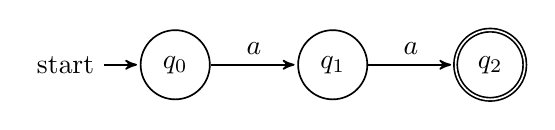
\begin{tikzpicture}[->,>=stealth',shorten >=1pt,node distance = 2cm,semithick]
  \tikzstyle{every state}=[text=black]

  \node[initial,state]   (Q0)                {$q_0$}; 
  \node[state]           (Q1) [right of=Q0]  {$q_1$}; 
  \node[state,accepting] (Q2) [right of=Q1]  {$q_2$}; 
  \path (Q0) edge node [above] {$a$} (Q1)

        (Q1) edge node [above] {$a$} (Q2);
\end{tikzpicture}
\label{fig:NFAaa}
\end{figure}

\label{fig:NFAaa}
\end{figure}

\begin{figure}
\centering
\caption{{\tt /ab/} NFA}
    \begin{figure}
\centering
\caption{{\tt /ab/} NFA}
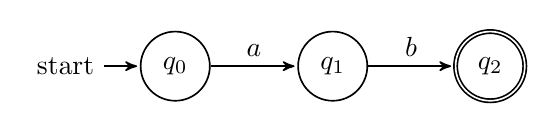
\begin{tikzpicture}[->,>=stealth',shorten >=1pt,node distance = 2cm,semithick]
  \tikzstyle{every state}=[text=black]

  \node[initial,state]   (Q0)                {$q_0$}; 
  \node[state]           (Q1) [right of=Q0]  {$q_1$}; 
  \node[state,accepting] (Q2) [right of=Q1]  {$q_2$}; 
  \path (Q0) edge node [above] {$a$} (Q1)

        (Q1) edge node [above] {$b$} (Q2);
\end{tikzpicture}
\label{fig:NFAab}
\end{figure}

\label{fig:NFAab}
\end{figure}


\begin{figure}
\centering
\caption{{\tt /aa/} $\cap$ {\tt /ab/} NFA}
    \begin{figure}
\centering
\caption{{\tt /aa/} $\cap$ {\tt /ab/} NFA}
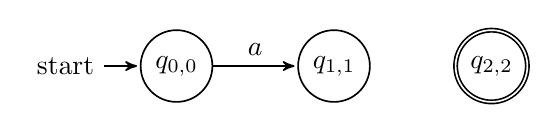
\begin{tikzpicture}[->,>=stealth',shorten >=1pt,node distance = 2cm,semithick]
  \tikzstyle{every state}=[text=black]

  \node[initial,state]   (Q00)                 {$q_{0,0}$}; 
  \node[state]           (Q11) [right of=Q00]  {$q_{1,1}$}; 
  \node[state,accepting] (Q22) [right of=Q11]  {$q_{2,2}$}; 
  \path (Q00) edge node [above] {$a$} (Q11)
        ;
\end{tikzpicture}
\label{fig:NFAaa:ab}
\end{figure}

\label{fig:NFAaa:ab}
\end{figure}

\begin{figure}
\centering
\caption{{\tt /a*/} NFA}
    \begin{figure}
\centering
\caption{{\tt /a*/} NFA}
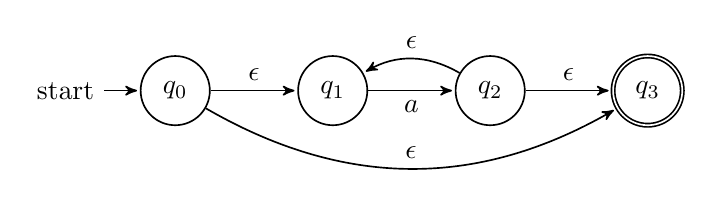
\begin{tikzpicture}[->,>=stealth',shorten >=1pt,node distance = 2cm,semithick]
  \tikzstyle{every state}=[text=black]

  \node[initial,state]   (Q0)                {$q_0$}; 
  \node[state]           (Q1) [right of=Q0]  {$q_1$}; 
  \node[state]           (Q2) [right of=Q1]  {$q_2$}; 
  \node[state,accepting] (Q3) [right of=Q2]  {$q_3$}; 
  \path (Q0) edge node [above] {$\epsilon$} (Q1)
             edge [bend right] node [above] {$\epsilon$} (Q3)

        (Q1) edge node [below] {$a$} (Q2)

        (Q2) edge node [above] {$\epsilon$} (Q3)
             edge [bend right] node [above] {$\epsilon$} (Q1)
        ;
\end{tikzpicture}
\label{fig:NFAastar}
\end{figure}


\label{fig:NFAastar}
\end{figure}

\begin{figure}
\centering
\caption{{\tt /aa/} $\cap$ {\tt /a*/} NFA}
    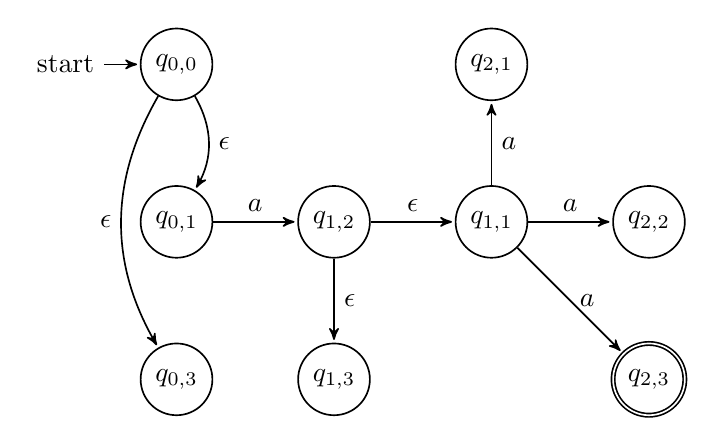
\begin{tikzpicture}[->,>=stealth',shorten >=1pt,node distance = 2cm,semithick]
  \tikzstyle{every state}=[text=black]

  \node[initial,state]   (Q00)                {$q_{0,0}$}; 
  \node[state]           (Q01) [below of=Q00] {$q_{0,1}$}; 
  \node[state]           (Q03) [below of=Q01] {$q_{0,3}$}; 

  \node[state]           (Q12) [right of=Q01] {$q_{1,2}$}; 
  \node[state]           (Q11) [right of=Q12] {$q_{1,1}$}; 
  \node[state]           (Q13) [below of=Q12] {$q_{1,3}$}; 

  \node[state]           (Q22) [right of=Q11] {$q_{2,2}$}; 
  \node[state]           (Q21) [above of=Q11] {$q_{2,1}$}; 
  \node[state,accepting] (Q23) [below of=Q22] {$q_{2,3}$}; 

  \path (Q00) edge [bend left]   node [right] {$\epsilon$} (Q01)
        (Q00) edge [bend right]  node [left] {$\epsilon$} (Q03)

        (Q01) edge node [above] {$a$} (Q12)

        (Q12) edge node [above] {$\epsilon$} (Q11)
        (Q12) edge node [right] {$\epsilon$} (Q13)

        (Q11) edge node [above] {$a$} (Q22)
        (Q11) edge node [right] {$a$} (Q23)
        (Q11) edge node [right] {$a$} (Q21)
        ;
\end{tikzpicture}

\label{fig:NFAaa:astar}
\end{figure}

\subsubsection{Regex Intersection on VM Instructions}

While regular expression intersection is most elegantly stated
in terms of abstract NFAs and the construction of an entirely
new automata, this approach needs to be modified if it is
to be used in the context of a VM NFA simulation. A regex
VM program is a representation of an NFA, but not in the usual
set-of-states and transition
table sort of way. Additionally, constructing an entirely
new NFA consumes space on the order of the product of the
size of the two input NFAs. Instead, we use the concept of
iterators, a primary warcry of the Rust programming language,
to provide the ability to explore a compound NFA without
ever materializing it. Rather than using a compiled
skip regex we use a regex compiled to use the unextended
set of VM instructions. This simplifies our job by reducing
the number of instructions we need to handle, and prevents
compiling skip instructions from recursively compiling any
subexpressions, which improves compiler performance.

To see how to decide the intersection of two NFAs described
by VM instructions, consider algorithm \ref{algo:regexinter}.
In the algorithm presented we use iterator generators
(expressed with the \verb'yield' keyword),
a feature common to programming languages which support coroutines
such as Python. Helper iterators over a single NFA are defined
in algorithm \ref{algo:nfaiter}. Rust does not yet support generators, so the
actual implementation instead uses explicit state machines, but
we use iterator generators here to make it easier to focus on the underlying
algorithm.

\begin{algorithm}
\caption{VM NFA Intersection} \label{algo:regexinter}
\begin{algorithmic}
\Procedure{NFAIntersectionIsEmpty}{$n_1$, $n_2$}
  \State Assume the existence of a $start$ function defined on
          VM programs which returns the starting instruction.
  \State Assume the existence of a $next$ function defined on
          VM program instructions which returns the next instruction
          in the program.
  \State $resume \gets [\langle start(n_1), start(n_2) \rangle]$
  \State $seen \gets \{\}$
  \While{$\langle s_1, s_2 \rangle \gets resume.pop()$}
    \If{$\langle s_1, s_2 \rangle \in seen$}
      \State \textbf{continue}
    \EndIf
    \State $seen \gets seen \cup \{\langle s_1, s_2 \rangle\}$
    \If{$s_1 = {\tt match} \wedge s_2 = {\tt match}$}
      \State \textbf{return} true
    \EndIf
    \State $resume.extend(IntersectChildren(s_1, s_2))$
  \EndWhile
  \State \textbf{return} false
\EndProcedure
\Procedure{IntersectChildren}{$inst_1$, $inst_2$}
  \For{$c1 \in$ Children($inst_1$)}
    \For{$c2 \in$ Children($inst_2$)}
      \Switch{$c1$}
        \Case{{\tt match}}
          \State \textbf{yield} $\langle c1, c2 \rangle$
          \State \textbf{break}
        \EndCase
        \Case{{\tt char} $\alpha_1$}
          \Switch{$c2$}
            \Case{{\tt match}}
              \State \textbf{yield} $\langle c1, c2 \rangle$
              \State \textbf{break}
            \EndCase
            \Case{{\tt char} $\alpha_2$}
              \If{$\alpha_1 \cap \alpha_2 \not= \emptyset$}
                \State \textbf{yield} $\langle c1, c2 \rangle$
              \EndIf
              \State \textbf{break}
            \EndCase
            \Case{default}
              \State unreachable
            \EndCase
          \EndSwitch
          \State \textbf{break}
        \EndCase
        \Case{default}
          \State unreachable
        \EndCase
      \EndSwitch
    \EndFor
  \EndFor
\EndProcedure
\end{algorithmic}
\end{algorithm}

\begin{algorithm}
\caption{VM NFA Iteration} \label{algo:nfaiter}
\begin{algorithmic}
\Procedure{Children}{$inst$}
  \State clear seen markings
  \Switch{$inst$}
    \Case{{\tt split L1 L2}}
      \State Terminals({\tt L1})
      \State Terminals({\tt L2})
      \State \textbf{break}
    \EndCase
    \Case{{\tt jmp L}}
      \State Terminals({\tt L})
      \State \textbf{break}
    \EndCase
    \Case{{\tt match}} \EndCase
    \Case{{\tt char} $\alpha$} \EndCase
    \Case{{\tt save} $s$}
      \State Terminals($next(inst)$)
      \State \textbf{break}
    \EndCase
  \EndSwitch
\EndProcedure
\Procedure{Terminals}{$inst$}
  \If{$inst$ is marked as seen}
    \State \textbf{return}
  \EndIf
  \State mark $inst$ as seen
  \Switch{$inst$}
    \Case{{\tt split L1 L2}}
      \State Terminals({\tt L1})
      \State Terminals({\tt L2})
      \State \textbf{break}
    \EndCase
    \Case{{\tt jmp L}}
      \State Terminals({\tt L})
      \State \textbf{break}
    \EndCase
    \Case{{\tt match}} \EndCase
    \Case{{\tt char} $\alpha$}
      \State \textbf{yield} $inst$
      \State \textbf{break}
    \EndCase
    \Case{{\tt save} $s$}
      \State Terminals($next(inst)$)
      \State \textbf{break}
    \EndCase
  \EndSwitch
\EndProcedure
\end{algorithmic}
\end{algorithm}

\section{Compiling without Optimization}
\label{section:compilation}

In this section, we define \verb'code', a compilation function mapping
from regular expressions to VM instructions. The approach taken here
draws heavy inspiration from Russ Cox's writeup of the virtual machine
approach to regular expressions (\cite{CoxVirtualMachineApproach}).
The \verb'code' function we present does not produce optimized code,
but serves as a baseline over which we will layer optimizations
in section \ref{section:skipscanopt}.
The \verb'code' function performs some simple case analysis on its
input and emits a recursively defined blob of code.
The particulars of this translation can
be found in table \ref{table:codedef}.

In the context of VM instructions, sets are written in
\texttt{SCREAMING\allowbreak\_SNAKE\allowbreak\_CASE}.
When a new label is mentioned in table
\ref{table:codedef} assume that it is fresh and unique as if it has
come from a \verb'gensym' like routine.

\begin{table}[ht]
\label{table:codedef}
\caption{Code Function}

\centering
\begin{tabular}{| l | l | p{8cm} |} \hline
Expression & Emitted VM Code & Discussion \\ \hline
$e_1 e_2$ &
  \begin{minipage}{3cm}
  \begin{verbatim}

code(e1)
code(e2)
  \end{verbatim}
  \end{minipage}
  & \\ \hline
$e_1 \rvert e_2$ &
  \begin{minipage}{3cm}
  \begin{verbatim}

split L1 L2
L1: code(e1)
    jmp L3
L2: code(e2)
L3:
  \end{verbatim}
  \end{minipage}
  & \\ \hline
$(e)$ &
  \begin{minipage}{3cm}
  \begin{verbatim}

save n
code(e)
save n+1
  \end{verbatim}
  \end{minipage}
  & 
  Here \verb'n' is given by $(i*2) + 2$ where $i$ is the index of
  the capture group being compiled in the regular expression. Slots $0$
  and $1$ are reserved for capturing the entire match, which is
  where the extra $2$ in the formula comes from. A nice corollary
  is that we can always know the number of slots that
  will be required ahead of time by computing $(c*2) + 2$
  where $c$ is the total number of capture groups.
  \\ \hline
$\epsilon$ & & The empty code block.  \\ \hline
$\alpha$ & \verb'char ALPHA' & Here \verb'ALPHA' is $\alpha$ \\ \hline
$e*$ &
  \begin{minipage}{3cm}
  \begin{verbatim}

split L1 L2
L1: code(e)
    split L1 L2
L2: 
  \end{verbatim}
  \end{minipage}
  & \\ \hline
$e+$ &
  \begin{minipage}{3cm}
  \begin{verbatim}

L1: code(e)
    split L1 L2
L2: 
  \end{verbatim}
  \end{minipage}
  & Note the way that $e+$ needs one less split instruction than $e*$. \\ \hline
$e*?$ &
  \begin{minipage}{3cm}
  \begin{verbatim}

split L2 L1
L1: code(e)
    split L2 L1
L2: 
  \end{verbatim}
  \end{minipage}
  & This is just like the result of \verb'code(e*)' except that the
    labels are flipped. \\ \hline
$e+?$ &
  \begin{minipage}{3cm}
  \begin{verbatim}

L1: code(e)
    split L2 L1
L2: 
  \end{verbatim}
  \end{minipage}
  & This is just like the result of \verb'code(e+)' except that the
    labels are flipped. \\ \hline
$.$ & \verb'char SIGMA' & Here \verb'SIGMA' is $\Sigma$. \\ \hline
\end{tabular}
\end{table}

\section{Core Optimizations}
\label{section:skipscanopt}

This section presents the key contribution of this thesis. If any of
these optimization patterns can apply, they are applied first, then
the remainder of the regex is compiled using the ordinary compilation
path. The applicability criterion for each optimization is discussed
below, and the relative precedence of different optimizations is
outlined in section \ref{section:optprecedence}.

 This section just covers the most common cases; a discussion of
how these common cases are extended to deal with minor semantic
variations can be found in section \ref{section:optextend}.

\subsection{Greedy Dotstar Scan}

The expression $.*l$ matches anything up to and including the first
appearance of $l$. The standard code emitted for this pattern involves
spawning two new threads, $t_1$ and $t_2$, for every character of input.
Thread $t_1$ tries to start matching the literal terminator, while thread $t_2$
accepts any and prepares to spawn another pair of threads.
Thread $t_1$ will keep dying until the first occurrence of $l$,
at which point it will try to match the rest of the regex.
Thread $t_2$ will keep rolling forward, splitting off threads that try
to match $l$, but if $t_1$ or any of its children match
$t_2$ will never execute due to its lower precedence.

Now consider an alternate compilation strategy, where $.*l$ is compiled
to:

\begin{verbatim}
L1: scan-end l
    split L1 L2
L2: 
\end{verbatim}

The above code will scan to the first occurrence of $l$, and then produce
one thread trying to match the rest of the expression and another that
keeps scanning forward for new occurrences of $l$. We claim that this
code behaves just as the standard approach does. The only way to
break out of either loop is to find an instance of $l$ in the input,
and in both cases the match is continued in just the same way. Thus,
while saving significant thread spawning overhead and allowing the use
of a very fast string searching algorithm such as Tuned Boyer-Moore, this
optimization will not change the results of the regex execution
(\cite{Hume1991}).

It might seem like we would be justified in applying a similar 
optimization to \verb'e*l', but this would allow matches to occur
when they ought not to. \verb'scan-end' will scan forward over anything
but $l$, but it would only be legitimate to scan forward over repetitions
of $e$, something which can only be determined with full execution of
the regular expression.

\subsection{Trailing $.*$}

If $.*$ or a similar expression appears at the end of a regular expression,
it is asking to scan forward to the end of the input rather than scan
forward until the next expression matches. Then any trailing $.*$ can
be safely compiled to:

\begin{verbatim}
goto-end
\end{verbatim}

To determine if an expression is in a trailing position we can 
invoke algorithm \ref{algo:marktrailing} on the top level expression
to recursively mark expressions as trailing. This annotation pass
informs us about when it is valid to apply the trailing $.*$ optimization.

\begin{algorithm}
\caption{Mark Trailing Expressions} \label{algo:marktrailing}
\begin{algorithmic}
\Procedure{MarkTrailing}{$expr$}
  \State mark $expr$ as trailing
  \Switch{$expr$}
    \Case{$e_1 e_2$}
      \State MarkTrailing($e_2$)
      \State \textbf{break}
    \EndCase
    \Case{$e_1 \rvert e_2$}
      \State MarkTrailing($e_1$)
      \State MarkTrailing($e_2$)
      \State \textbf{break}
    \EndCase
    \Case{$e*$}
    \EndCase
    \Case{$e*?$}
    \EndCase
    \Case{$e+$}
    \EndCase
    \Case{$e+?$}
    \EndCase
    \Case{$(e)$}
      \State MarkTrailing($e$)
      \State \textbf{break}
    \EndCase
    \Case{$\epsilon$}
    \EndCase
    \Case{$\alpha$}
    \EndCase
    \Case{$.$}
    \EndCase
  \EndSwitch

  \Comment{Note that while MarkTrailing($e_1 e_2$) marks the outer
            concatenation expression as trailing, the inner expressions
            are marked separately so that $e_1$ is not marked as trailing
            and $e_2$ is.}
\EndProcedure
\end{algorithmic}
\end{algorithm}

\subsection{Literal-Terminated Scan}
\label{section:littermscan}

If an expression containing no capture groups is followed by a
literal or set of literals, it might be possible to just scan forward
to find that literal. It is possible to scan forward to find a literal
terminator with Tuned Boyer-Moore (\cite{Hume1991}) or a hardware
accelerated approach (\cite{GallantRegex}) and a group of literal
terminators using Aho-Corasick (\cite{Aho1975}) or Teddy (\cite{Teddy}).
For simplicity we just discuss scan optimization for expressions of
the form $el$, but it can just as easily apply to expressions of the
form $e(?:l1|l2|...|)$ or $e(l1|l2|...|)$.
If $L(.*l.*) \cap L(e) = \emptyset$ and $e$ does
not contain captures, then $l \not\in L(e)$\footnote{The details of deciding
this problem are laid out in section \ref{section:regexinterdecide}.}.
Thus we know that the first occurrence of $l$
in the input will not be part of the input which matches $e$. That means
it is legitimate to compile $el$ to:

\begin{verbatim}
scan-end l
\end{verbatim}

The idea of this optimization is straightforward, but ensuring that
it is applied to maximum effect requires a little more thought. There
are two main concerns. First, if two or more literals appear in an
expression we want to scan to the last one if possible. It wouldn't
do to process the expression from left to right because then we could
end up scanning forward to each literal when some could be skipped over
entirely. Second, if a literal appears in a concatenation of expressions
we want to make sure that the largest possible group of expressions
is skipped over. To accomplish these goals we can replace the approach
to compiling a concatenation of expressions given by the definition of
\verb'code' with algorithm \ref{algo:optconcat}.

\begin{algorithm}
\caption{Optimizing Concatenation} \label{algo:optconcat}
\begin{algorithmic}
\Procedure{CompileConcatOpt}{$e_1 ... e_n$}
  \For{$i \in n..i$}
    \If{$e_i$ is a literal we can scan to}
      \For{$j \in 0..i$}
        \If{$e_j ... e_{i-1} \cap .*i_i.* = \emptyset$}
          \Comment{This means we can scan to $e_i$}
          \State emit CompileConcatOpt($e_1 ... e_{j-1}$)
          \State emit \verb'scan' $e_i$
          \State emit code($e_{i+1} ... e_n$)
          \State \textbf{break}
        \EndIf
      \EndFor
      \State \textbf{break}
    \EndIf
  \EndFor
  \If{there were no literals in $e_1 ... e_n$}
    \State emit code($e_1 ... e_n$)
      \Comment{Give up on the optimization.}
  \EndIf
\EndProcedure
\end{algorithmic}
\end{algorithm}

Note that in reality, the logic for the $el$ optimization must be
interleaved with the logic for the $.*l$ optimization, so the
real concatenation compiler routine is more complicated. For
expository purposes we consider them separately.

\subsection{Skip}
\label{section:skipopt}

The idea of the skip optimization is to compile a literal, $l$, to

\begin{verbatim}
skip len(l)
\end{verbatim}

The trouble is that just skipping over literals won't work at choice points.
To illustrate the problem, consider the regex \verb'/ac(.).|bc.(.)/'
on the input \verb'bcxy', which demonstrates a few different problems with
just compiling literals to skips.

% The first issue is that we will miss situations where literals are
% concatenated with other expressions with a statically known length.
% In this case $bc$ is concatenated with \verb|'.'|. To address this
% we implement logic which will attempt to compute the
% length of regular expressions. Any regular expression with a
% known length is then compiled into a skip.

The second issue is that there is no way to make sure that the
thread from a non-matching branch dies if the input fails to match in
the middle of a skip. By assumption, we know that the overall regular
expression matches, but we have no guarantee that any particular branch
matches. In the case of \verb'/ac(.).|bc.(.)/' on \verb'bcxy' the
first capture group parsed would be \verb'x' rather than \verb'y' as
it should be. The first thread has higher precedence and would
fail to die because the skip avoids looking at the \verb'a' char.
To resolve this issue we need a special compilation path for skips
that begin on the branches of a choice point. Examples of
choice points are the alternative operator ($\rvert$),
and the repetition operators ($*$, $+$, $*?$, $+?$).

Rather than compile to just a skip instruction, branches
at a choice operator have to compile to a char instruction
followed by a skip instruction.

\begin{verbatim}
char FIRST_SET
skip n-1
\end{verbatim}

Here \verb'FIRST_SET' is the set of characters which might
begin the regular expression ($fset(e_{branch})$).
Even this guard is not valid if the first sets of any two
branches at the branch point intersect. For example it would
not help deal with $a(.).|a.(.)$. In such cases we give up
on the optimization entirely.

\section{Optimization Variants and Extensions}
\label{section:optextend}

Section \ref{section:skipscanopt} outlines the most basic and most
important optimizations based on the \verb'skip' and \verb'scan-end'
instructions. There is, however, more to the story.
Real regular expression libraries provide several different repetition
operators, and the best way to leverage scan instructions to optimize
repetitions must take into account considerations around capture groups and
precedence.

% TODO: skip fusion
%While skipping over raw literals, and making sure to avoid
%falling prey to subtle ambiguities is important, we can do better.
%Both \verb'xxx' and \verb'xxx|yyy' ought to compile down to
%the same \verb'skip 3' instruction.

\subsection{Scan Variants}

\subsubsection{Lazy Dotstar Scan} %: {\tt code}($.*?l$)}

$.*?l$ gets compiled to:

\begin{verbatim}
L1: scan-end l
    split L2 L1
L2: 
\end{verbatim}

This optimization follows similar logic to that used for the greedy
dotstar optimization. At first it might appear that we would be able
to dispense with the non-determinism for the lazy variant, as laziness
means that we are after the shortest possible match so we don't
need to keep looking for future terminators. Unfortunately, there
might be a match failure in the expression which follows the
\verb'.*?'. More concretely, consider the regular expression
\verb'/.*?term(?:x)(.)/'
to be executed on \verb'aaaatermbbbbbbtermxy'. The correct solution will
capture the \verb'y' character, but without a non-deterministic branch
after the scan the scanning thread will just find the first terminator and
die. Thus, we still need non-determinism even in the lazy case.

\subsubsection{Capture Terminated Greedy Dotstar Scan}
  \label{capterm}

If there is a capture group around the literal we are scanning forward
for, we need to grab that capture. $.*(l)$ gets compiled to:

\begin{verbatim}
L1: scan-start l
    save n
    skip len(l)
    save n+1
    split L1 L2
L2: 
\end{verbatim}

\subsubsection{Capture Terminated Lazy Dotstar Scan}

If the repetition was lazy the operands to split are flipped.
$.*?(l)$ get compiled to:

\begin{verbatim}
L1: scan-start l
    save n
    skip len(l)
    save n+1
    split L2 L1
L2: 
\end{verbatim}

\subsubsection{Dotplus Scan}

All the optimizations for dotstar scanning also apply to dotplus
patterns (i.e. $.+l$). One might be concerned that the literal scan
might accidentally find its literal right at the start of the input,
something which should not be allowed because $.+$ demands at least
one character of input be consumed before the match can proceed.
Fortunately, the partial parsing assumption saves us. The input must
be in the language of the regex we are parsing, so there will always
be at least one leading character to scan over.

\subsection{Skip Extensions}

\subsubsection{Skip Choice: {\tt code}($e1 \rvert \dots \rvert en$)}

Section \ref{section:skipopt} already introduced the idea that
compiling skips at choice points requires a bit of extra thought.
This section goes into a more detail about how exactly skips are
handled in the context of an alternative.
This optimization applies iff none of the first sets of $e1 \dots en$
intersect. If they do intersect, we have to fall back on the standard
compilation strategy. Note that we can't just define this operation as
an optimization over a binary operator because we need a view of each
of the branches.

\begin{verbatim}
split L1 L2
L1: branch_code(e1)
    jmp LEND
L2: split L2ENTER L3
L2ENTER: branch_code(e2)
         jmp LEND
L3: split L3ENTER L4
L3ENTER: branch_code(e3)
         jmp LEND
...
LN: branch_code(en)
LEND:
\end{verbatim}

Here \verb'branch_code' behaves just like \verb'code' except 
for the differences outlined in table \ref{table:branchcode}.
Unless otherwise noted where \verb'code' recursively calls
itself, \verb'branch_code' recursively calls \emph{itself}
(the one exception is that tail of a concatenation is
compiled with the standard \verb'code' function).
The \verb'branc_code' function boils down to compiling literals
as a \verb'char' followed by a \verb'skip' rather than just
a \verb'skip', and making sure to do so recursively through
the structure of the expression.

\begin{table}
\caption{Differences Between Branch Code and Code}
This represents a modification to table \ref{table:codedef}.
\label{table:branchcode}
\centering
\begin{tabular}{| l | l |} \hline
Input Expression & Emitted VM Code \\ \hline
$l e$ &
  \begin{minipage}{4cm}
  \begin{verbatim}

char fset(l)
skip (len(l) - 1)
code(e)
  \end{verbatim}
  \end{minipage}
  \\ \hline
$l$ &
  \begin{minipage}{4cm}
  \begin{verbatim}

char fset(l)
skip (len(l) - 1)
  \end{verbatim}
  \end{minipage}
  \\ \hline
$e_1 e_2$ &
  \begin{minipage}{4cm}
  \begin{verbatim}

branch_code(e1)
code(e2)
  \end{verbatim}
  \end{minipage}
  \\ \hline
\end{tabular}
\end{table}
 
\subsubsection{Greedy Skip Star}

If the first sets of $e1$ and $e2$ don't intersect, $e1*e2$
is compiled as:

\begin{verbatim}
split L1 L2
L1: branch_code(e1)
    split L1 L2
L2: branch_code(e2)
\end{verbatim}

Where \verb'branch_code' is defined by table \ref{table:branchcode}.
The lazy variant just flips the split operands. If the first
sets to intersect, unoptimized code must be generated. The story
is really a little more complex because we have to consider
expressions of the form $e1*e2*...en$. In such cases, we much
check to see if any of the first sets of $e1$, $e2$, and $en$.

\subsubsection{Greedy Skip Plus}

If the first sets of $e1$ and $e2$ don't intersect.

\begin{verbatim}
L1: branch_code(e1)
    split L1 L2
L2: branch_code(e2)
\end{verbatim}

Where \verb'branch_code' is defined by table \ref{table:branchcode}.
The lazy variant just flips the split operands. Multiple
repeated expressions are handled just as they are for
Kleene star.

\section{Optimization Precedence}
\label{section:optprecedence}

When an optimization can be applied, it is, but when multiple
mutually exclusive optimizations can be applied, one must be
selected. While we have not defined a rigorous cost model
to do optimization selection, we do have some heuristics.
Our goal is to skip or scan over as much input as possible.
While skipping has the most potential for speedup, we
believe that scans are more likely to quickly consume large
chunks of input. Most literals are relatively small, while
it is quite a bit more common to see \verb'.*' used to eat
up large chunks of input. The $el$ optimization has the
potential to scan over the most preceding subexpressions\footnote{
Keep in mind that $e$ might be a concatenation.},
so we give it the highest precedence. The trailing \verb'.*' optimization
can never conflict with another optimization, so we don't have to
assign it a precedence. All that remains is the order of the \verb'.*l'
optimization and the literal skip optimization. If we gave the
literal skip optimization a higher precedence, the \verb'.*l'
optimization would never trigger. Additionally, the \verb'.*l'
optimization includes skipping over the literal terminator.
Then there is no reason to place the literal skip optimization
at a higher precedence. Table \ref{table:optprec} defines these
precedence levels concisely.

\begin{table}
\caption{Optimization Precedence}
\label{table:optprec}

\centering

\begin{tabular}{| c | c |} \hline
Optimization & Precedence Level (lower applies first) \\ \hline
\verb'el' & 1 \\ \hline
\verb'.*l' & 2 \\ \hline
Literal Scan & 3 \\ \hline
Trailing \verb'.*' & n/a \\ \hline
\end{tabular}
\end{table}

% TODO: why?
% \subsubsection{Fixed Length Skip: {\tt code}($s$)}
% 
% It is important that this optimization have lower precedence
% than the other skip optimizations. Here \verb's' is an
% expression with a statically known length.
% 
% \begin{verbatim}
% scan len(s)
% \end{verbatim}

\chapter{An Implementation}
\label{chapter:implementation}

This chapter details our implementation of a regular expression
engine which leverages skip regex. We implemented skip regex as
an extension to rust's Regex crate. The decision to extend rather
than start a fresh project allowed us to reuse the parser,
testing tools, and even a few implementation techniques. Extending
an existing library made it even easier to provide backwards
compatibility with an existing ecosystem. Our implementation
can be found at \verb'https://github.com/ethanpailes/regex/tree/skip-regex'.
% TODO: pin to a specific commit or release tag before publication.

%% Talk about use cases??

\section{Architecture}

Executing a skip regular expression requires a number of phases
arranged in a pipeline. Before any work can be done on the regex,
it must be parsed. Fortunately, the backwards compatible concrete
syntax of skip regex means that we could just use the parser provided
by rust's regex crate. The real work of executing skip regex does not
pick up until it is time to compile the regular expression.

Skip regex are compiled by applying the \verb'code' function defined
in the Compilation section. In practice, we make a few adjustments to
the compilation technique for performance. The biggest such change
is to the format of the VM instructions that we execute. Rather than
using explicit labels, each instruction is annotated with one or
two \verb'goto' pointers indicating the next instruction to jump to.
This enables the complete removal of the \verb'jmp' instruction, which
cuts down on both code size and the number of cycles required to execute
a particular regex. This new format requires continually back-patching
the last instruction or instructions that were compiled, which is a bit
less clear than the direct style used to define the \verb'code' function.
% TODO: reference Compilation section properly when I stitch these
%       things together

Once a regular expression is compiled, it can be executed by one
of many potential engines, each with its own set of trade offs.
The main engine we use is a bounded backtracking engine. The
implementation is covered in greater detail below, but the core
idea of a bounded backtracker is to extend a standard backtracker
with a bitset indicating which states the engine has already
been in. So long as history does not matter (which is the case
when back-references are not allowed), it is safe to skip any
state which has already been visited. Doing so has the benefit
of restoring guaranteed linear running time.

The bitset that allows the bounded backtracker to provide guaranteed
linear running time is $O(|input||regex|)$ in space, which is
cheap when the regex and input are small but can get quite expensive
as they grow. Rob Pike's lockstep VM does not suffer from this
space blowup, so it makes a good fallback despite running slower
for small cases. Unfortunately, Pike's VM cannot handle branch
precedence correctly when extended with the ability to execute
skip instructions. Match disambiguation is not always required,
so this does not completely negate the usefulness of Pike's VM
when extended with skip instructions (\cite{Pike1987}).

\section{Backwards Incompatibilities or Missing Features}

The Rust regex library is a mature and full featured regular expression
engine. This provided significant opportunity to reuse well tested
components, but it also meant that bringing a new regex engine to
full feature parity with the existing pipeline was difficult. We
choose to defer implementation of a few features that the regex crate
supports in order to focus on exploring the key concepts in play.
We discuss these features briefly here to provide a sketch of how
they might be added to skip regex.

The first feature we omit is support for case-insensitive regex.
Many regex engines provide a flag which asks the engine to ignore
case when performing a match. This is useful when searching for
words embedded in natural language or keywords of a case-insensitive
language like SQL. Implementing this feature can be performed as
an AST rewrite pass, where each character is replaced by a character
class which includes both the character and its capitol version.
For example \verb'abc' would be rewritten as \verb'[aA][bB][cC]'.
Implementing this flag as an AST transform had a bit of an
impedance mismatch with the version of the regex crate that we
forked, but there is no reason it should not work with skip regex.

The second feature we omit is unicode support. Unicode support in
a regex library is non-trivial, primarily due to the fact that
unicode code-points are variable width. This makes indexing into
a unicode string $O(n)$ in the size of the string. The scan optimizations
on skip regex would be unaffected by this, because they have to deal
with scanning forward over chunks of the input anyway. Even in the
context of a unicode string, substring search algorithms can operate at
the byte level. The implementation of the skip instruction would require
a bit more work. The simplest thing to do would be to just construct
a unicode DFA to decode the input, and then use it to scan quickly
forward. This would take the runtime of the skip instruction from
$O(1)$ to $O(n)$, but the constant factor would still be lower
than the cost associated with an NFA simulation. We could improve on
this situation significantly by adding a separate \verb'skip-exact'
instruction for use in situations where the size in bytes of the
skip can be statically determined. Thus, a literal unicode character
which takes up three bytes would compile down to a \verb'skip-exact 3'
instruction. Adding support for unicode to skip regex would be significantly
more work than adding support for case folding, but would still be
perfectly feasible.

\section{Skip Bounded Backtracker}

The primary backend used to execute skip regex is the skip bounded
backtracker. Backtracking regex engines have a long history.
Their speed, ease of implementation, and extensibility make them
a great choice for a regex backend, but they suffer from a worst-case
exponential running time. This exponential blow up can be fixed by
keeping a bitset which tracks every state that the engine has
ever been in, where a state is identified by the tuple of the
instruction pointer and the input index. Once the engine has
been in a particular state once, there is no need to explore it
again.
% TODO: cite Russ Cox?

The primary cost associated with the bounded backtracker is
the initialization of the bitset, which consumes $O(|regex||input|)$
space. Very few executions cause the NFA simulation to enter all
or most states, but initializing the bitset to all zeros must always
touch every state bit. When the expression and input are small, the
cost is negligible, but as they grow it eventually starts to dominate.
All of the skip regex optimizations we perform have the effect of
reducing code size, which cuts down on the size of the bitset,
and hence the cost of its initialization.

\subsection{Algorithm}

The bounded backtracking algorithm can be very naturally expressed
in terms of a recursive function parameterized by a set of captures,
an instruction pointer, and a string offset.  The ``Backtrack'' procedure
laid out in algorithm \ref{algo:recurboundedback} takes an array of capture
slots, an instruction pointer and a string pointer as input and returns
either ``NoMatch'' to indicate that no match could be found
or ``Match($captures$)'' to indicate that there was a match with the
given capture slots. Some pre processing is required to
set up the bitset (here called $seen$) and the capture slots,
and some post processing is required to convert the capture slots
to capture groups suitable for user consumption, but the core
of the algorithm is here. Strictly speaking, ``Backtrack'' should
never return ``NoMatch'' because it is invalid to invoke a skip
regex on input which will not match the regex, but the concept of
a failed intermediary match is required to support non deterministic
branching internally (the \verb'split' instruction). There are also
some cases where skip regex \emph{can} detect invalid input at no
extra cost, and there is no particular reason to avoid telling the
user about such cases.

Algorithm \ref{algo:recurboundedback} is still presented at a
high level, and there are a number of tricks that we use in the
real implementation which improve performance at the cost of
readability. We use an explicit bitset rather than an abstract
set to implement the seen-set. Rather than using explicit recursion,
we use a heap-allocated stack of actions representing stack frames.
We avoid copying the $captures$ array at every step by modifying
a single captures array in place and introducing a restoration action
which can be interleaved with the standard stack resumption action.
Similarly, the instruction pointer and string pointer are modified
in place. Algorithm \ref{algo:loopboundedback} implements these
optimizations. Several of the less interesting instructions are
omitted for brevity, but it should be easy to see how the implementation
might be translated form algorithm \ref{algo:recurboundedback}

\begin{algorithm}
\caption{Recursive Bounded Backtracker} \label{algo:recurboundedback}
\begin{algorithmic}
\State Assume the existence of a $scan\_to\_start(needle, haystack)$ function
        which performs fast substring search for the needle in the haystack
        (using Tuned Boyer-Moore, or hardware accelerated literal search
        as appropriate).
\State Let $input$ be the input string.
\State Let $insts$ be the instructions.
\State $seen \gets \{\}$
\Procedure{Backtrack}{$captures$, $ip$, $sp$}
  \If{$\langle ip, sp \rangle \in seen$}
    \State \textbf{return} NoMatch
  \EndIf
  \State $seen \gets seen \cup \{\langle ip, sp \rangle\}$
  \Switch{$insts[ip]$}
    \Case{{\tt split L1 L2}}
      \Switch{Backtrack($captures$, {\tt L1}, $sp$)}
        \Case{NoMatch}
          \State \textbf{return} Backtrack($captures$, {\tt L2}, $sp$)
        \EndCase
        \Case{Match($captures'$)}
          \State \textbf{return} Match($captures'$)
        \EndCase
      \EndSwitch
    \EndCase
    \Case{{\tt jmp L}}
      \State \textbf{return} Backtrack($captures$, {\tt L}, $sp$)
    \EndCase
    \Case{{\tt match}}
      \State \textbf{return} Match($captures$)
    \EndCase
    \Case{{\tt skip} $n$}
      \State \textbf{return} Backtrack($captures$, $ip + 1$, $sp + n$)
    \EndCase
    \Case{{\tt save} $s$}
      \State $captures[s] \gets sp$
      \State \textbf{return} Backtrack($captures$, $ip + 1$, $sp$)
    \EndCase
    \Case{{\tt char} $\alpha$}
      \If{$sp < input.len() \wedge input[sp] \in \alpha$}
        \State \textbf{return} Backtrack($captures$, $ip + 1$, $sp + 1$)
      \Else
        \State \textbf{return} NoMatch
      \EndIf
    \EndCase
    \Case{{\tt scan-end} $l$}
      \If{$literal\_start \gets scan\_to\_start(l, input[sp..])$}
        \State \textbf{return}
            Backtrack($captures$, $ip + 1$, $literal\_start + len(l)$)
      \Else
        \State \textbf{return} NoMatch
      \EndIf
    \EndCase
    \Case{{\tt scan-begin} $l$}
      \If{$literal\_start \gets scan\_to\_start(l, input[sp..])$}
        \State \textbf{return}
                  Backtrack($captures$, $ip + 1$, $literal\_start$)
      \Else
        \State \textbf{return} NoMatch
      \EndIf
    \EndCase
    \Case{{\tt goto-end}}
      \State \textbf{return} Backtrack($captures$, $ip + 1$, $input.len()$)
    \EndCase
  \EndSwitch
\EndProcedure
\end{algorithmic}
\end{algorithm}

\begin{algorithm}
\caption{Bounded Backtracker} \label{algo:loopboundedback}
\begin{algorithmic}
\State Let $input$ be the input string.
\State Let $insts$ be the instructions.
\Procedure{Backtrack}{$inst\_p$, $string\_p$}
  \State $seen \gets \{\}$
  \State $resume \gets [State(inst\_p, string\_p)]$
  \State $captures \gets [NONE, ...]$
  \While{$r \gets resume.pop()$}
    \Switch{$r$}
      \Case{$State(ip, sp)$}
        \If{$\langle ip, sp \rangle \in seen$}
          \State \textbf{break}
        \EndIf
        \State $seen \gets seen \cup \{\langle ip, sp \rangle\}$
        \While{$sp < input.len()$}
          \Switch{$insts[ip]$}
            \Case{{\tt split L1 L2}}
              \State $resume.push(State(L2, sp))$
              \State $ip \gets L1$
              \State \textbf{break}
            \EndCase
            \Case{{\tt match}}
              \State \textbf{return} true
            \EndCase
            \Case{{\tt skip} $n$}
              \State $sp \gets sp + n$
              \State $ip \gets ip + 1$
              \State \textbf{break}
            \EndCase
            \Case{{\tt save} $s$}
              \State $resume.push(Restore(s, captures[s]))$
              \State $captures[s] \gets sp$
              \State $ip \gets ip + 1$
              \State \textbf{break}
            \EndCase
            \Case{{\tt char} $\alpha$}
              \If{$input[sp] \in \alpha$}
                \State $ip \gets ip + 1$
                \State \textbf{break}
              \Else
                \State \textbf{return} false
              \EndIf
            \EndCase
            \Comment{Some cases omitted}
          \EndSwitch
        \EndWhile
        \State \textbf{return} false
      \EndCase
      \Case{$Restore(slot, val)$}
        \State $captures[slot] = val$
        \State \textbf{break}
      \EndCase
    \EndSwitch
  \EndWhile
\EndProcedure
\end{algorithmic}
\end{algorithm}

\section{Skip PikeVM}

While it is usually not as fast as the bounded backtracker,
a modified version of Rob Pike's lockstep VM (\cite{Pike1987})
can also be used to execute skip regex. The skip Pike VM cannot
implement greedy vs lazy match differentiation, so it can't be
used in situations where this is important. Because of these
limitations relative to the skip bounded backtracker, we will
try to keep our discussion of the skip Pike VM brief\footnote{
Russ Cox provides an in depth discussion of the Pike VM style
of NFA simulation (\cite{CoxVirtualMachineApproach}).
}.

The core idea of a Pike VM is to maintain two sets of threads:
one situated at the current character and one at the next character.
In a standard NFA simulation, no thread will ever spawn with
a string pointer in any location besides these two, and
neither set of pending threads can ever grow larger than
the number of instructions, as duplicate threads are ignored.
Such a scheme requires a representation of a set of threads
between $0$ and $|regex|$ in size that supports fast containment
checking, fast iteration, and fast clearing. A sparse set using
uninitialized memory makes all of these operations constant except
for iteration which is linear (\cite{Briggs1993}), which makes it
a good choice for the representation of a thread set. This
effectively limits the number of steps which can occur
at any character of input to be $O(|regex|)$, guaranteeing that
the runtime does not exceed $O(|regex||input|)$. Typically the regex
is small, so this can be thought of as linear in the size of the input.

In order to support skip regex, the Pike VM must be able to deal
with threads in more than two locations. This requires expanding
the queue of runnable threads beyond a couple of just thread sets.
It is tempting to place all threads in a priority queue where
priority is determined by location in the input and precedence,
but this approach would cause the running time to become
$O(|regex||input|lg(|regex||input|))$, as retrieving the highest
priority thread would become logarithmic in the number of
of potential runnable threads rather than being constant.

To retain the algorithmic properties demanded by the runqueue,
we instead use a fixed size ring buffer of sparse sets, with
each set containing threads $n$ characters forward in the input,
where $n$ is the distance from the current sparse set. This means
that skips further ahead in the input than the length of the ring
buffer cannot be executed in one step, but we observe that most
skips are smaller than $60$, the ring buffer size that we choose
through benchmarking. It is more common for scan instructions to
require being repeatedly deferred to the furthest forward sparse set,
but we still observe a speedup in such cases.

Figure \ref{fig:pikeexecchar} contains an example that walks though
the representation of threads as the Pike VM steps through a simple
program that decides the regex \verb'/a/'. Here threads are represented as
a 2-tuple of an instruction pointer and an array of capture slots.
There is no need to store a string pointer because the thread set
which contains a thread implies its offset into the string.
Instructions like \verb'save' do not advance the string pointer,
so the first step of the Pike VM pops $t_0$, executes save instruction
by saving the current string pointer to the first capture slot, then
pushes a new thread, $t_1$, to the current thread set. The second step
does advance the string pointer, so when $t_1$ is transformed into $t_2$
it is pushed to the thread set at index 1 instead of index 0.

Figure \ref{fig:pikeexecskip} contains an example that walks through
the execution of a simple program containing the \verb'skip' instruction.
This demonstrates the ability to jump forward in the input, by pushing
a new thread to one of the thread sets further ahead in the ring buffer.
In such a case the skip Pike VM will notice that intermediate thread
sets are empty, and quickly skip over them.

\begin{figure}
\caption{Executing a {\tt char} Instruction in the skip Pike VM}
\centering
\label{fig:pikeexecchar}

\begin{tabular}{ l l }
\textbf{Instructions} &
  \begin{tabular}{| r | l |}
  \hline
  Index & Instruction \\ \hline
  0 & \verb'save 0' \\ \hline
  1 & \verb'char a' \\ \hline
  2 & \verb'save 1' \\ \hline
  2 & \verb'match' \\ \hline
  \end{tabular} \\ \\
\textbf{Step 0, Thread Set Index = 0} &
  \begin{tabular}{| c | c | c | c |}
  \hline
  $t_0 = \langle 0, [NONE, NONE] \rangle$ & & & \\ \hline
  \end{tabular} \\ \\
\textbf{Step 1, Thread Set Index = 0} &
  \begin{tabular}{| c | c | c | c |}
  \hline
  $t_1 = \langle 1, [0, NONE] \rangle$ & & & \\ \hline
  \end{tabular} \\ \\

\textbf{Step 2, Thread Set Index = 0} &
  \begin{tabular}{| c | c | c | c |}
  \hline
  & $t_2 = \langle 2, [0, NONE] \rangle$ & & \\ \hline
  \end{tabular} \\ \\

\textbf{End of Thread Set 0} & \\ \\

\textbf{Step 3, Thread Set Index = 1} &
  \begin{tabular}{| c | c | c | c |}
  \hline
  & $t_3 = \langle 3, [0, 1] \rangle$ & & \\ \hline
  \end{tabular} \\ \\

\textbf{Match} & \\

\end{tabular}
\end{figure}

\begin{figure}
\caption{Executing a {\tt skip} Instruction in the skip Pike VM}
\centering
\label{fig:pikeexecskip}

\begin{tabular}{ l l }
\textbf{Instructions} &
  \begin{tabular}{| r | l |}
  \hline
  Index & Instruction \\ \hline
  0 & \verb'save 0' \\ \hline
  1 & \verb'skip 3' \\ \hline
  2 & \verb'save 1' \\ \hline
  2 & \verb'match' \\ \hline
  \end{tabular} \\ \\
\textbf{Step 0, Thread Set Index = 0} &
  \begin{tabular}{| c | c | c | c |}
  \hline
  $t_0 = \langle 0, [NONE, NONE] \rangle$ & & & \\ \hline
  \end{tabular} \\ \\
\textbf{Step 1, Thread Set Index = 0} &
  \begin{tabular}{| c | c | c | c |}
  \hline
  $t_1 = \langle 1, [0, NONE] \rangle$ & & & \\ \hline
  \end{tabular} \\ \\

\textbf{Step 2, Thread Set Index = 0} &
  \begin{tabular}{| c | c | c | c |}
  \hline
  & & & $t_2 = \langle 2, [0, NONE] \rangle$ \\ \hline
  \end{tabular} \\ \\

\textbf{End of Thread Set 0} & \\ \\

\textbf{End of Thread Set 1} & \\ \\

\textbf{End of Thread Set 2} & \\ \\

\textbf{Step 3, Thread Set Index = 3} &
  \begin{tabular}{| c | c | c | c |}
  \hline
  & & & $t_2 = \langle 2, [0, 3] \rangle$ \\ \hline
  \end{tabular} \\ \\

\textbf{Match} & \\

\end{tabular}
\end{figure}

\chapter{Evaluation}
\label{chapter:evaluation}

In order to be worthwhile, skip regex must be faster than standard
regex and there must be ample opportunity to apply them. To evaluate
the degree to which skip regex meet these goals, we perform a number
of experiments.  We present a series of micro benchmarks to demonstrate
the performance of skip regex under specific conditions. The micro
benchmarks show that the performance of skip regex is
at least as good as the equivalent standard regex execution, and 
is often significantly better. To determine the usefulness of skip
regex for regular expressions found in the wild, we scraped
\verb'crates.io', the Rust package repository,
for regular expressions and tested to see how applicable each of the 
optimizations we perform are. Finally, we perform a case study walking
through the steps a programmer might take while parsing logs from
an Apache Kafka instance.

\section{Microbenchmarks}

Microbenchmarks alone are not typically enough to develop a high
level understanding of application performance, yet they remain
quite useful for demonstrating performance edge cases. Put another
way, microbenchmarks are excellent tools for performance story
telling. Sometimes such story telling can be used to deceive,
but we will attempt to avoid any deception and instead focus
on the performance trade-offs of skip regex.

% TODO: explain methodology.
The micro benchmarks we present in this section each consist of
a regex template and an input template which get instantiated
based off of some scaling factor and then run with different
backends. The scaling factor typically increases the input
size by a constant number of characters, and less commonly
increases the regex size. We run each microbenchmark at a
number of different scaling factors using Rust's built in
benchmarking facility, which takes a number of samples before
reporting the average runtime plus the spread between the minimum
and maximum runtime. We indicate the spread by attaching error bars to
each datapoint in our scatter plots.

In order to demonstrate the utility of different optimizations,
we execute the benchmarks with different engines and different
optimizations enabled. The standard regex engines are called
\texttt{baseline\allowbreak -\allowbreak backtrack} and
\texttt{baseline\allowbreak -\allowbreak pike}, while the
skip backends are called \texttt{skip\allowbreak -\allowbreak backtrack}
and \texttt{skip\allowbreak -\allowbreak pike},
with a number of optimization specifiers tacked onto the end to
indicate which optimizations have been enabled. For example,
\texttt{skip\allowbreak -\allowbreak backtrack\allowbreak -\allowbreak
        ds\allowbreak -\allowbreak es\allowbreak -\allowbreak sl}
indicates that the skip backtracker with $.*$ scanning, $e*$ scanning,
and literal skipping enabled.

% TODO: open up a documentation PR so that other people don't
%       have to go digging through rustc source to figure out
%       what the +/- means.

\subsection{Best Possible Case: A Big Skip}

The best possible case for skip regex is where a regex is composed
entirely of large literals. In such a case a standard regex engine
must laboriously test ever input character, while a skip regex
engine is allowed to traverse the input in a few big hops. Figure
\ref{fig:a:big:skip} illustrates just such a case. Here we executed the
regex \verb'/aaaa(bbbb)cccc/' on an input of the form \verb'aaaabbbbcccc'.
In both the regex and the input, the number of \verb'a' and \verb'c'
characters was multiplied by the scaling factor. As we might expect,
the graph shows that both the skip Pike VM and the skip backtracker
beat out the non-skip backtracker quite handily, with the running time
of the skip engines remaining virtually flat as the running
time of the standard backtracker grows linearly with the scaling factor.
The performance improvement is entirely due to the literal skip
optimization, as shown by the fact that the performance of the skip
backtracker with literal skipping disabled matches the
\verb'baseline-backtrack' configuration.

\begin{figure}
\label{fig:a:big:skip}
\caption{A Big Skip}

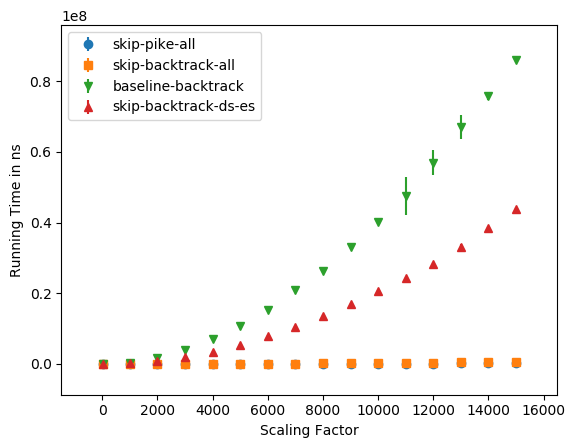
\includegraphics{resources/a-big-skip.png}
\end{figure}

\subsection{Leading $.*$}

While not quite as good as being able to traverse the whole input
in a few hops, a leading $.*$ which can be scanned over to find the
correct terminator after the first try is still very fast. A standard
regex must go through the expensive process of spawning two new threads
for each character of input, one of which will die after each step.
By contrast, a skip regex engine can drop right into a fast substring
search algorithm. We produced figure \ref{fig:leading:dotstar} by executing
\verb'/.*(aaaa)/' on \verb'baaaa' with \verb'b' repeated according
to the scaling factor. The graph shows that all the engines are linear
in the size of the input, but the constant factor for the skip engines
is so much lower that they appear nearly constant time.

\begin{figure}
\caption{Leading $.*$}
\label{fig:leading:dotstar}

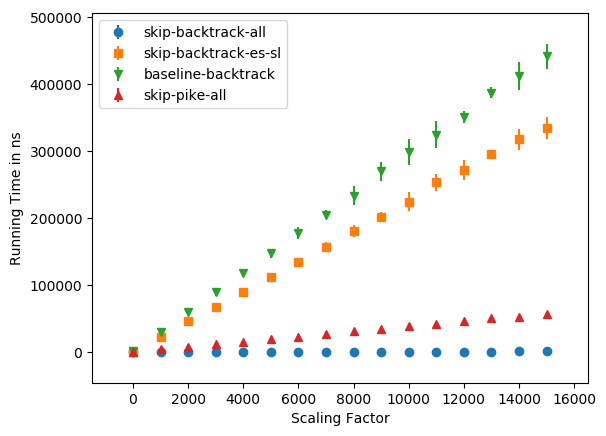
\includegraphics{resources/leading-dotstar.png}
\end{figure}

\subsection{$.*$ Bounce}

It would not be fair to showcase the best possible case for the
$.*$ scan optimization without also demonstrating the worst
case. If the literal terminator appears many times before the
end of the repetition, the skip engine will be forced to
rapidly enter and leave the substring search algorithm, spawning
two new threads on every iteration. This essentially makes
the dotstar scan optimized code no better than a standard regex
execution. To demonstrate this worst case situation we executed
the regex \verb'/.*a(bbbb)/' on \verb'cabbbb' with \verb'ca'
repeated according to the scaling factor. Figure \ref{fig:dotstar:bounce}
shows that the skip backtracker is slower than the standard
backtracker due to the overhead of switching back and forth between the
literal searcher and main engine loop. When the $.*$ optimization is
turned off, the skip backtracker behaves just like the standard
backtracker. This example was constructed to showcase the worst
case for the $.*$ scan optimization, but it seems less likely to appear
in the wild than the best case.

\begin{figure}
\caption{$.*$ Bounce}
\label{fig:dotstar:bounce}

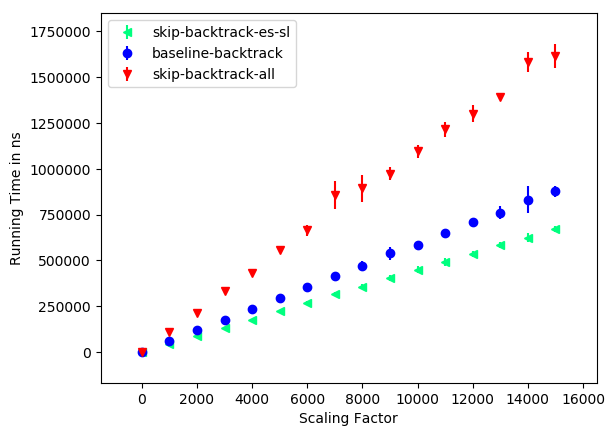
\includegraphics{resources/dotstar-bounce.png}
\end{figure}

\subsection{Leading $e*$ scan}

The other scan optimization only really has a best case, because
the scan is always guaranteed to find the literal terminator. The
effectiveness of the optimization is entirely determined by the
size of the input, something which can be completely described
by one experiment. We produced figure \ref{fig:leading:noncontaining:estar}
by executing the regex \verb'a*foo(bar)' on \verb'afoobar' with \verb'a'
repeated according to the scaling factor. Just as in the ``Leading $.*$''
experiment, all engines are linear, but the skip backends are so much
faster that they appear almost constant time.

\begin{figure}
\caption{Leading $e*$}
\label{fig:leading:noncontaining:estar}

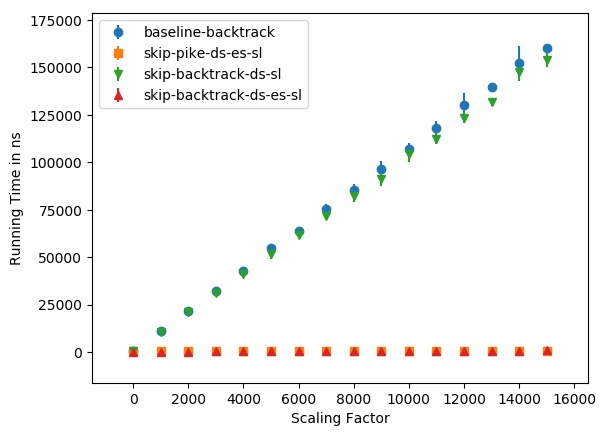
\includegraphics{resources/leading-noncontaining-estar.png}
\end{figure}

\subsection{No Opt}

In some cases no optimizations can be usefully applied to a skip
regex. We include such a case to demonstrate that with the exception
of a bouncing $.*$ optimization, the performance of skip regex is
no worse than that of standard regex. We produced figure 
\ref{fig:justtwo:branch}
by executing the regex \verb'/(ab|ac)*/' on \verb'ab' with
the input multiplied by the scaling factor. The fact that the
two branches of the alternative have intersecting first sets
(in particular $\{a\}$ and $\{a\}$), means that skip optimizations
can't be applied, and there is no clever way to get out of
executing the full kleene star. There is still some spread between
the different engines, most notably between the Pike VMs and the
bactrackers, as backtrackers are generally faster. The skip Pike VM
has a higher constant factor than the standard Pike VM when optimizations
are not helping out because of the increased complexity of its runnable
thread queue. The skip backtracker seems to have a slightly better
constant factor than the standard backtracker for this benchmark.
This difference may come from some slight overhead associated with
unicode support\footnote{Unicode support is turned off for the
standard backtracker in this benchmark, but the code is written
to be generic over both unicode and byte-oriented input, which
may come at a cost.}.

\begin{figure}
\caption{No Opt}
\label{fig:justtwo:branch}

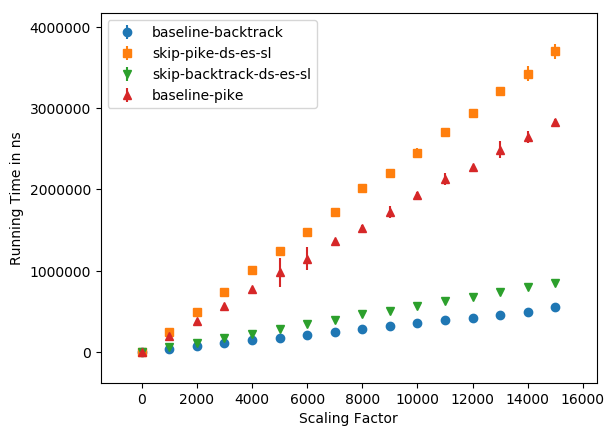
\includegraphics{resources/justtwo-branch.png}
\end{figure}

\section{Log Parsing: A Case Study}

Regular expressions can be used in core application code, but they
are quite frequently used in a more improvisational capacity.
Searching through source code in an editor, filtering and parsing
the output of a previous command in a unix pipeline, and aiding
the construction of quick one-off scripts are all examples of
common use cases for regular expressions. We present an example
walking through the use of skip regex in pre-validated mode
to scrape an Apache Kafka debug log file. This case study
demonstrates the utility of skip regex beyond the library context
illuminated by the \verb'crates.io' figures presented in section
\ref{section:applicability}.

\subsection{Experimental Setup}

Apache Kafka is a Java-based distributed queuing system with
named event categories called topics consisting of several
queues called partitions. Like many network applications,
Kafka contains extensive and configurable debug logging,
which makes it a good source of test data. We configured
Kafka to log as promiscuously as possible and used a simple
python script to repeatedly publish and consume from a 
\verb'test' topic. We used the resultant log file as input
to our scraping script. To make the input log large enough
to observe a difference in performance, we concatenated the
log to itself several times.

The code for our program can be found at \cite{PailesSkipRegexCaseStudy},
but its usage message is worth including here to make
interpreting the invocations we used for our experiments
easier.

\begin{verbatim}
Usage: scrape [options] <log-file>
       scrape -h

Options:
    -v, --validate  First filter with a DFA, then apply skip regex.
    -a, --append    Summarize the append events.
    -n, --named     Summarize the named events.
    -h, --help      Print this help message.
\end{verbatim}

\subsection{Summarizing Append Events}

When a new message is appended to a Kafka log it notes some
metadata about the message such as its size and the offset to
which it was written in the partition. To get a summary of
the append events that occurred in a particular log we 
determine the minimum and maximum offsets appended to,
as well as the total number of append events and the total
number of bytes written. We used the regex
\verb'^.* with first offset: ([0-9]+).*value=([0-9]+).*$'
to extract the offset and the total number of bytes from append
log lines. When we executed our program in first standard mode
then skip mode we got the following output.

\begin{verbatim}
scrape$ du -h server.log
25M     server.log
scrape$ time ./target/release/scrape -a server.log 
3900/111098 (3.51%) append events
1000 min offset
1299 max offset
58110 total bytes written

real    0m0.128s
user    0m0.117s
sys     0m0.012s
scrape$ time ./target/release/scrape -a -v server.log 
3900/111098 (3.51%) append events
1000 min offset
1299 max offset
58110 total bytes written

real    0m0.097s
user    0m0.091s
sys     0m0.006s
\end{verbatim}

Note that because only 3.51\% of lines matched, most of the time
was spent in the DFA discarding non-matching lines in both cases.
The \verb'0.026' second difference in user time then comes from
the 3900 matching lines. When we stripped away the non-matching
lines to more directly observe the difference in performance
of the two NFA simulations we got the following results.

\begin{verbatim}
scrape$ cat server.log | rg "with first offset:" > appends.log 
scrape$ du -h appends.log 
848K    appends.log
scrape$ time ./target/release/scrape -a server.log 
3900/111098 (3.51%) append events
1000 min offset
1299 max offset
58110 total bytes written

real    0m0.129s
user    0m0.120s
sys     0m0.009s
scrape$ time ./target/release/scrape -v server.log 

real    0m0.029s
user    0m0.022s
sys     0m0.007s
\end{verbatim}

This shows that there is significant difference in the performance
of the NFA simulations, and highlights the value of using the DFA
to filter out non-matching lines even for a standard NFA simulation
approach.

\subsection{Counting Named Events}

Kafka has a number of named tasks that can be used to track
the behavior of the server. In order to extract the names
of these events we used the regex 
\texttt{/.* \allowbreak scheduled \allowbreak task \allowbreak '(.+?)'.*\$/}
To find out which events happened most frequently, we built
a histogram and then printed out a summary of the ten most
common events. We ran our scraping script first with the standard regex
backend, and then with our skip regex backend in validation
mode. This produced the following output.

\begin{verbatim}
scrape$ du -h server.log 
25M     server.log
scrape$ time ./target/release/scrape -n server.log 
28262/111098 (25.44%) named events
event isr-change-propagation happened 12844 times.
event isr-expiration happened 6422 times.
event highwatermark-checkpoint happened 6422 times.
event kafka-recovery-point-checkpoint happened 546 times.
event kafka-log-start-offset-checkpoint happened 546 times.
event kafka-delete-logs happened 546 times.
event transaction-abort happened 520 times.
event kafka-log-retention happened 130 times.
event auto-leader-rebalance-task happened 130 times.
event delete-expired-group-metadata happened 78 times.

real    0m0.225s
user    0m0.220s
sys     0m0.004s
scrape$ time ./target/release/scrape -n -v server.log 
28262/111098 (25.44%) named events
event isr-change-propagation happened 12844 times.
event isr-expiration happened 6422 times.
event highwatermark-checkpoint happened 6422 times.
event kafka-recovery-point-checkpoint happened 546 times.
event kafka-log-start-offset-checkpoint happened 546 times.
event kafka-delete-logs happened 546 times.
event transaction-abort happened 520 times.
event kafka-log-retention happened 130 times.
event auto-leader-rebalance-task happened 130 times.
event delete-expired-group-metadata happened 78 times.

real    0m0.122s
user    0m0.115s
sys     0m0.007s
\end{verbatim}

A quarter of the log lines were about named events, so the speedup
from using skip regex was much more noticeable for this case.

\section{Applicability}
\label{section:applicability}

It is hard to evaluate the applicability of the optimizations presented
in this thesis. It is quite easy to invent scenarios where each
optimization might be worthwhile, so any such examples alone are
suspect. Existing regular expressions provide a better tool for
evaluating applicability, but it is important to watch out for
bias towards one particular application in any sample of existing
regex. It is also important to consider the fact that skip regex
can be used as more than just a faster regex engine. In situations
where a programmer might otherwise be inclined to directly encode
skips and scans to quickly parse some trusted input, they can
instead write skip regex with the intent of triggering optimizations.
Such optimization-aware usage cannot be evaluated by examining
existing regex.

A nice thing about extending an existing regex engine
with a decently sized user base is that a diverse group of developers
have written all sorts of different regex using the existing syntax.
In order to compile a list of such regex we pulled down all the
crates on \verb'crates.io' which depend on the regex crate, and
searched their source code for occurrences of the pattern
\verb'Regex::new\((r?".*")\)'. This only collected a subset of
the regex that could possibly be found, as there are ways to
produce a Rust regex without calling \verb'Regex::new', but
other methods of construction are unusual.

Once we had collected
a list of 487 regex, we ran them though our compiler, taking
note whenever an optimization was triggered. We found that
82.8\% of regex could have some sort of skip optimization
applied. 74.1\% of regex could have a literal compiled to a skip,
but only 6.5\% could have a $.*$ optimization applied and 8.6\% could
have a $e*$ optimization applied. 15.0\% could have some sort of
scan optimization applied. It is heartening to see that most regex
can benefit from skip optimizations, though the relatively low number
of opportunities for scan optimizations is less so. While skip
optimizations have the greatest potential for speedup\footnote{By turning
a linear time operation into a constant time one.}, most skips
are relatively short.

It is worth taking these numbers with a grain of salt. \verb'crates.io'
is very library heavy, which likely biases the dataset towards
more complex and tricky regex. The more complex a regex gets,
the more opportunity for first set collisions there are, which gets
in the way of optimization. The sorts
of regex used to scrape log files or extract data in a unix pipeline
are more likely to have a linear feel than the regex found in
libraries. As an example, the regex we used to convert the output
of \texttt{cargo \allowbreak bench}, Rust's benchmarking utility, to a machine
readable CSV format was
\texttt{/test \allowbreak([a-zA-Z:\_]+) \allowbreak +... bench\allowbreak
      : \allowbreak+([0-9,]+) \allowbreak ns/iter \textbackslash
      (\textbackslash+/\textbackslash- \allowbreak
      ([0-9,]+)\textbackslash).*\$/}
This regex contains multiple different opportunities for skip optimizations,
but is not really general enough to put in a library. Contrast this
with the regex
\texttt{
/([0-9a-zA-Z]\allowbreak\{1\}\allowbreak/\allowbreak
[0-9a-zA-Z]\{1\}\allowbreak[:]\allowbreak\{1\})
\{5\}\allowbreak[0-9a-zA-Z]\allowbreak{1}\allowbreak[0-9a-zA-Z]
\allowbreak\{1\}/
}
found in the \verb'wifiscanner' crate, which does not allow for
optimization. It is possible for a one-off data munging script to include
such a complex regex, and for a library to include a simple one, but
it seems less likely. It is also worth noting the size of the corpus of
regex we collected. 487 is a large enough number to get 
percentages worth talking about, but it is not as large as it might
be for a more mature language ecosystem.

% TODO: discussion of skip regex time complexity

\chapter{Related Work}
\label{chapter:relatedwork}

\section{Some Regex History}

Regular expressions have a dual history as both a theoretical
and practical tool. Any regular expression corresponds to an
NFA which decides its language, and thanks to a
result from Rabin and Scott (\cite{Rabin1959}) we know that
these NFAs can be translated into equivalent DFAs. The powerset
construction they provide trades a potentially exponential runtime
blowup for a potentially exponential space blowup.
The exponential runtime vs exponential space tradeoff,
is often the end of the story as presented in CS curricula,
but for the regex implementer it is only the beginning. Both
naive NFA simulation and naive DFA construction are potentially exponential
in some respect. Even worse, DFAs created via the powerset construction
cannot support features like capture groups and back references 
which programmers have come to expect in a regular expression engine.

The story of modern regex tools is the story of trying to grapple
with the tradeoffs and capabilities of NFA vs DFA approaches.
The lineage of the current generation of regular expression tools
can be traced back to an implementation which compiled
to PDP-11 machine code provided by Thompson (\cite{Thompson1968}).
Thompson's work involved compiling directly to machine code, but
future iterations on his work instead targeted virtual instruction
sets and provided VM interpreters (\cite{CoxVirtualMachineApproach}).
The two primary contributions of Thompson's paper were a translation
from a regular expression to an NFA and a guaranteed linear time
NFA simulation. Ironically, the first contribution is most commonly 
remembered despite the fact that the paper spills very little ink
on it and devotes most of its space to linear time simulation.
It was really Aho, Hopcraft, and Ullman who formalized the regex to NFA
translation as ``Thompson's Construction'' in a series of 
publications, most notably ``The Design and Analysis of Computer Algorithms''
(\cite{Aho1974}). The thread based approach that Thompson pioneered
forms the basic paradigm on which skip regex build.

The next chapter in regex tooling is about adding pragmatic text
processing features. Building off of Thompson's work,
Rob Pike added capture groups to the flavor of regular expressions
he included in his Sam text editor (\cite{Pike1987}). Larry Wall's
Perl programming language, released in 1987, included a builtin
regular expression facility (\cite{Perl}). Perl's regular
expressions included capture groups and back references, the
latter feature actually making them non-regular. In order to
support these features Perl's regex engine gave up on guaranteed
linear time execution. Perl's backtracking NFA
simulation was easier to implement, faster than Thomson's VM in most
cases, and easier to add features to. The success of Perl and its
emphasis on using regular expressions for text processing quickly
lead to a proliferation of backtracking regex engines (\cite{PCRE},
\cite{PCRE2}, \cite{Python}, Java, Javascript). The primary
project of skip regex is making the submatch extraction feature
pioneered by these engines more efficient.

Backtracking NFA simulations had come to dominate the regular
expression landscape outside of theoretical circles by the
time that Russ Cox began work on executing untrusted regular
expressions\footnote{Regular expressions provided by unknown
or untrusted users.}. On the face of it, regular expressions with their
restricted semantics seem like a reasonable thing to expose to
untrusted users, but any backtracking implementation will inevitably
be vulnerable to a DOS attack in the event that a malicious user
provides a pathological regular expression. In order to
overcome this issue Russ Cox wrote RE2, a library
which focuses on reclaiming guaranteed linear time execution (\cite{CoxRE2}).
Like Perl before it, RE2 inspired other regex engines to
follow its design philosophy, the most prominent of which are
Rust's regex library (\cite{GallantRegex}) and go's regex library
(\cite{GoLang}). Skip regex are committed to avoiding an
exponential runtime blowup by leveraging Cox's techniques.

\section{Current Research}

While capture groups were often part of regex implementations,
they were not a main focus of study until Ville Laurikari laid
out a submatch extraction algorithm with guaranteed linear time
and space (\cite{Laurikari2001}). Laurikari's main contribution
was the notion of a tagged NFA transition, essentially converting
regex NFAs to transducers which accumulate captured text as they
work. Laurikari's tagged transitions are closely related to the
\verb'save' instruction found in many regex VM implementations
(\cite{CoxVirtualMachineApproach}). The guaranteed linear
running time of Laurikari's tagged NFAs makes them an excellent
candidate for the sort of adversarial regex execution that RE2
and its decedents aim to facilitate. Skip regex build off of
the tagging approach by re-using the idea of saving string offsets
with special instructions.

Sulzman and Lu provide a regex submatch extraction algorithm
based on the concept of regular expression differentiation
(\cite{Sulzmann2012}). Rather than using a flavor of Thompson's
Construction as all of the approaches touched on so far have done,
their work is based off of a Glushkov automata (\cite{Allauzen2006}).
An implementation of their algorithm in Haskell was as fast or
faster than other native Haskell implementations, and competitive
with C implementations. Sulzman and Lu's work relies on
Antimirov's partial regular expression derivatives (\cite{Antimirov1996}),
an extension of Brzozowski regular expression derivatives
(\cite{Brzozowski1964}). Regex differentiation with respect
to an input character involves stripping that character from
the leading portion of the regex. For example the regex \verb'/ab/'
differentiated with respect to the character \verb'a' is \verb'/b/'.
Similarly, the regex \verb'/ab|ac/' differentiated with respect to
\verb'a' is \verb'/b|c/'. This notion is closely related to the
idea of first-sets which are key to determining when
the skip optimizations presented in this thesis are safe to perform.

Substring search, the problem of finding a shorter string (the needle) in
a longer string (the haystack), is a simpler problem than regular expression
matching, and one that can be solved much faster. The family of fast substring
search algorithms known as Boyer-Moore all involve some pre-processing of
the needle to enable sub-linear running time (\cite{Boyer1977}).
The subject of substring search is very closely studied, leading to
endless variations on the core algorithm Robert Boyer and J Moore
first presented. Fortunately for the uninitiated, Andrew Hume and
Daniel Sunday performed a comprehensive review of the substring search
literature, providing a clean taxonomy of substring search algorithms
and a recommendation to use a variant called Tuned Boyer-Moore
(\cite{Hume1991}). Theoretically ideal asymptotic complexity is not,
however, the end of the story. When we implemented Tuned Boyer-Moore,
we found that it was seldom able to beat a simpler approach based on
frequency analysis and the \verb'memchr' function already found in
the \verb'regex' crate (\cite{GallantRegex}). On Intel machines this
difference boils down to the use of the \verb'pcmpeqb' instruction,
which allows multiple bytes to be checked at once
(\cite{IntelInstructionManual}); other platforms have their own hardware
acceleration for substring search. Fast substring search is crucial to
the scan optimizations of skip regex. Without the use of fast substring
search, the results of this thesis would be considerably weaker.

While not quite as fast as pure substring search, the multiple
substring search problem can also be decided quite a bit faster than
full regex matching. In particular the Aho-Corasick algorithm provides
fast multiple substring search (\cite{Aho1975}). Just like Boyer-Moore,
Aho-Corasick loses out to a hardware accelerated variant despite its
theoretical elegance. The accelerated algorithm, called Teddy, seems
to have first appeared in the hyperscan regex library (\cite{hyperscan}),
and was reverse-engineered and illuminated in the Teddy library (\cite{Teddy}).
The most important take-away is that substring and multiple
substring search are quite a bit faster than full regular expression matching.
We use multiple substring search for scan optimizations just as we do for
single substring search.

Haber provides an efficient DFA based submatch extraction algorithm,
which managed to get significant runtime speedups at the cost of
increased compile time work (\cite{Haber2013}). The algorithm uses
a deterministic finite transducer run backwards over the input
to produce a stream of states. A second automata uses these
states as input and is ultimately responsible for constructing
the capture groups. Compilation is quite expensive, potentially
going exponential and requiring the construction of four separate
automata (two of which are intermediate automata that are quickly
thrown out). Being a DFA approach, the algorithm suffers from
a potentially exponential blowup in the size of the DFA just as
the subset construction does, but this situation seldom arises.
Unfortunately, due to the extreme compile time cost of this
approach, it seems unlikely that the exponential blowup can be
remedied by lazy compilation as is typically done for the subset
construction. The ability to compute capture groups with
just DFAs represents a significant advancement in the state of the art.

Howard Chivers provides a series of optimizations over standard NFA
simulation approaches based on the notion of a regular expression preview
(\cite{Chivers2016}). For any regex $r$, there exists a preview $p_n$
such that $L(p_n) \supseteq \{ w[0..n] | w \in L(r) \}$. In English,
an $n$-preview will recognize the first $n$ characters
of a match, but it might turn up some false positives. The thing that
makes previews useful as an optimization tool is that they can be
decided with very simple DFAs, which enjoy much faster execution than
the NFA simulation that Chivers embedded them in. Previews provide
a quick way to fail fast before committing to a non-deterministic
branch, and a good way to find candidate locations to attempt a
full parse. In this way, previews bear a lot of similarities to the
scan optimizations presented in this thesis. In fact, previews can be
viewed as a generalization of literal scanning. They are completely
compatible, and indeed complementary with the work presented in this
thesis.

% TODO: Briggs (An Efficient Representation of Sparse Sets)

% TODO: Talk about one-pass DFAs

\chapter{Future Work}
\label{chapter:futurework}

There is significant opportunity for skipping over more complicated
expressions than just literals. The simplest case is skipping over
alternatives where each branch is of the same length. A more interesting
problem is adding AST rewrite passes which factor common prefixes and
suffixes out of alternatives in order to increase the length of skips.
For example \verb'/a(?:bbc|bbyx)/' might could be rewritten as
\verb'/abb(?:c|yx)/'.

Both the skip regex optimizations presented in this thesis and
Chivers' notion of previews (\cite{Chivers2016}) represent
extensions to the VM approach to NFA simulation. The approaches
are compatible, so it would be interesting to see how an engine
which makes use of both sets of optimizations performs. Beyond
just being compatible with skip regex, regex previews have
synergistic potential with them. In particular, previews make
it possible to quickly scan forward to a point which might begin
any regex, which ought to allow an expansion of the cases where
the scan optimizations presented in this thesis are applicable.

It would be nice to add support for unicode and case folding to
the skip regex engine, as this would allow skip regex to be used
as a truly drop-in replacement for the Rust regex crate\footnote{
When used in conjunction with a DFA to filter out non-matching
input}.

The original motivation for investigating parsing a regex without
deciding it was the need to perform a partial parse for the PADS
language. Now that the problem of partial parsing has been worked
out for regular expressions, a natural next step is to see how
the work extends to a language like PADS. Of particular interest
is the ability to decide when two PADS grammars have an empty
intersection. PADS grammars tend to have a bit more structure
than regex, so it seems like the $e*$ optimization has more
potential than the $.*$ scan optimization. The ability to check
if two pads grammars have an empty intersection is a key piece
of analysis for enabling such an optimization. Another angle
to consider is the fact that PADS grammars are not regular,
which opens up the potential for optimizations. To scan
forward over a parenthesized s-expression something like
algorithm \ref{algo:sexpscan} seems to be the
optimal solution. This sort of counting scan can't come up
in the context of regular expressions due to their regularity,
but it must be considered for PADS.

\begin{algorithm}
\caption{S-Exp Scan} \label{algo:sexpscan}
\begin{algorithmic}
\Procedure{SExpScan}{$i$}
  \State $num\_parens \gets 0$
  \State $in\_quote \gets false$
  \While{true}
    \If{$input[i] = '('$}
      \If{$\neg in\_quote$}
        \State $num\_parens \gets num\_parens + 1$
      \EndIf
    \ElsIf{$input[i] = ')'$}
      \If{$\neg in\_quote$}
        \State $num\_parens \gets num\_parens - 1$
      \EndIf
    \ElsIf{$input[i] = '"'$}
      \State $in\_quote \gets \neg in\_quote$
    \EndIf
    \State $i \gets i + 1$
    \If{$num\_parens = 0$}
      \State \textbf{break}
    \EndIf
  \EndWhile
  \State \textbf{return} i
\EndProcedure
\end{algorithmic}
\end{algorithm}

% TODO: to facilitate optimization-aware programming I should make it
%       easier to understand when a particular optimiztion is applied.

\chapter{Conclusion}
\label{chapter:conclusion}

The primary objectives of this thesis were the production of a
fast and useful implementation of regular expression parsing,
and laying theoretical groundwork for future work in partial
parsing.

We examined the performance profile of skip regex in detail
using microbenchmarks, and provided application level performance
numbers through case studies. Both types of benchmarks suggest
that skip regex can produce a speedup over existing
implementations. The case studies we present provide examples
of how skip regex might be applicable, but to further
the claim of applicability we show that over 80\% of regex
found on \verb'crates.io' can benefit from some sort of
skip optimization.

In addition to being a suitable replacement for standard
regex with the help of a DFA filter, skip regex open up
a new approach to programming. Programmers have long made
the distinction between trusted and untrusted binary data.
Skip regex provide a systemic approach to handling trusted
textual data. The usefulness of this distinction is hard to
evaluate without giving programmers time to use the new tool,
but the existence of the analogous distinction with respect to
binary data is promising.

This thesis uncovered a number of insights that ought to be
useful for examining partial parsing in the context of PADS.
We have shown that while substring search is in the same complexity
class as regular expression parsing, the difference in constant
factors is so huge that looking for opportunities to scan forward
to some literal is very important. The work on analyzing the
ambiguity at branch points and checking for regex intersection
ought to be useful when attempting to analyze PADS grammars
for optimization.

Skip regex are fast, applicable to real applications, open
up a new approach to programming with trusted text, and lay
the groundwork for further work in partial parsing.


%================================ END of chapters =============================

\addcontentsline {toc}{chapter}{Bibliography}
                                     %% Force Bibliography to appear in contents

%\begin{thebibliography}{..}          %% Start your bibliography here; you can
%\bibitem{...} ...                    %% also use the \bibliography command
%\end{thebibliography}                %% to generate your bibliography.

\bibliographystyle{alpha}
\bibliography{thesis}

%\begin{thesisauthorvita}             %% Write your vita here; it can be
%...                                  %% anything in LaTeX2e par-mode.
%\end{thesisauthorvita}               %%

\end{document}                       %% Done.
